\chapter{Design of an Observing System Simulation Experiment for the Operational Model of the Southwestern Coast of Iberia (SOMA)} \label{sec:cp2}
\vspace{\fill}
\textbf{Article reference}:\\
Mendonça, F., Martins, F., \& Bertino, L. (2025). Design of an Observing System Simulation Experiment for the Operational Model of the Southwestern Coast of Iberia (SOMA). \textit{Journal of Marine Science and Engineering}, 13(9), 1830. \href{https://doi.org/10.3390/jmse13091830}{https://doi.org/10.3390/jmse13\\091830}
\newpage

\section{Abstract}
Observing System Simulation Experiments (OSSEs) provide a framework in which to evaluate the impact of prospective ocean-observation networks on model forecasting performance prior to their actual deployment. This study presents the design and validation of an OSSE tailored for the operational coastal model of southern Portugal, SOMA. The system adopts the fraternal twins approach and a univariate data-assimilation scheme based on Ensemble Optimal Interpolation to update the model's 3D temperature structure with SST. The methodology provides a flexible framework that preserves the statistical structure of real observation errors while remaining independent of SOMA. This allows straightforward transfer to other applications, thereby broadening its applicability and making it useful as a starting point in the design of observation networks beyond that presented in this case study. The OSSE experiments were compared against corresponding Observing System Experiments (OSEs) using real satellite SST products. Results show that the designed OSSE is internally consistent, sensitive to observation density, and capable of reproducing realistic correction patterns that closely match those obtained in the OSEs. These findings provide strong evidence that the SOMA OSSE system is a reliable tool for assessing the potential impact of future surface-observation strategies.

\vspace{15mm}
\noindent\textbf{Keywords}: coastal model; ocean observation; data assimilation; ensemble optimal interpolation; observation experiments
\vspace{10mm}

\section{Introduction} \label{sec:ossedesign_intro}
Numerical modelling is one of the primary tools used for understanding and predicting marine system dynamics. Hydrodynamic models simulate the ocean state by translating the physics of fluid motion into a computational framework that approximates the solution of discretized primitive equations using numerical methods \parencite{versteeg2007introduction, griffies2006some}. These methods are implemented as algorithms that advance the ocean state forward in time over a defined spatial domain. Through this process, models enable the simulation of oceanic conditions, providing valuable insights into the structure and evolution of marine systems under both natural variability and anthropogenic influence.

While numerical models are essential in ocean prediction, they are still only one element of the broader framework used to understand marine systems in operational oceanography. Observations lie at the centre of the scientific method and provide the factual basis needed to develop and validate theoretical formulations and numerical models. It is primarily through the continuous and systematic observation of ocean phenomena via in-situ measurements, remote sensing, or other monitoring technologies \parencite{letraon2011satellites} that empirical knowledge of the ocean's dynamics is established. Historical data collected on water variables provide critical information about climate evolution, such as changes in sea surface height (SSH) \parencite{frederikse2020causes, gomez2024satellite} and variations in water temperature \parencite{mills2024baseline, liu2023twenty}.

The observation network is a cornerstone of operational oceanography and has driven increasing demand for high-quality oceanographic data. As a result, the evolution of observation-system technologies has enabled real-time measurements of various ocean variables \parencite{legler2015current, letraon2015use}. Despite this progress, observational data often present significant spatial and temporal gaps, particularly in remote or logistically challenging regions. Because the implementation of new ocean-observation systems typically involves substantial financial investment and technical complexity, Observing System Simulation Experiments (OSSEs) provide a framework in which to evaluate the potential impact of additional observations before their actual deployment by exploring hydrodynamic models and data assimilation (DA) systems \parencite{prive2023robustness}.

The purpose of an OSSE system is to ensure that the additional observations will meaningfully contribute to scientific and operational goals. However, since it relies on synthetic data (Section 3), the development of such a system requires using an Observing System Experiment (OSE) to serve as a benchmark by which to validate the OSSE \parencite{halliwell2014Rigorous}. While both approaches operate in a similar manner, OSEs rely on real-world, existing observations to evaluate their impact through data denial experiments, comparing model performance with and without specific datasets. Demonstrating that an OSSE system produces impact assessments consistent with those of an OSE, researchers confirm the credibility of the framework for evaluating future observing systems. This validation step is critical to ensuring the system produces realistic and reliable predictions before resources are committed to new observational deployments.

Within this context, the NAUTILOS project \parencite{novellino2022new} is focused on developing cost-effective next-generation technologies for ocean observation. Funded by the Horizon 2020 program of the EU's Future of Seas and Oceans Flagship Initiative, the project addresses critical gaps in marine monitoring, particularly for chemical, biological, and deep-ocean physical variables. By integrating innovative sensors and samplers into a range of ocean platforms, such as autonomous vehicles, mooring buoys, and fisheries-observation systems, the project contributes to a standardized, interoperable system for marine data collection, enhancing global efforts to understand and manage ocean ecosystems. Aligned with the broader goals of the NAUTILOS project, the present work focuses on the development and validation of an OSSE system tailored to an operational hydrodynamic model of the southern coast of Portugal. The primary objective is to establish and verify the functionality of the OSSE system itself, ensuring that it is capable of supporting future assessments of observational strategies.

The subsequent sections are structured to present the key components and methodologies adopted in the development of the proposed OSSE system. Section \ref{sec:ossedesign_algarve} outlines the main oceanographic features of the Algarve region, the focus of this study. Next, Section \ref{sec:ossedesign_osse} provides a comprehensive overview of the OSSE framework, while Section \ref{sec:ossedesign_da} presents the general formulation of the Ensemble Optimal Interpolation (EnOI) scheme, which was used as the DA method in the designed system. Building on this context, the OSSE system was implemented for the Algarve Operational Modeling and Monitoring System (SOMA), a hydrodynamic model based on MOHID, as described in the first part of the methodology (Section \ref{sec:ossedesign_method}). The second part details the design choices made for the system, including a fraternal twins configuration of SOMA, which was used to represent two distinct model realizations for comparative assessment. It also describes how observations are extracted from the system and the implementation of the EnOI scheme in SOMA. Finally, Section \ref{sec:ossedesign_results} and Section \ref{sec:ossedesign_conclude} present the results of the system's implementation and the main conclusions of this work.

\section{Algarve General Circulation} \label{sec:ossedesign_algarve}
The south of Iberia is characterized by a Mediterranean climate, which features distinct seasonal variations with hot, dry summers and mild, humid winters. The average annual temperature in this region is approximately 17$^\circ$C, with summer temperatures frequently exceeding 22$^\circ$C and reaching maximums around 40$^\circ$C. In contrast, winter temperatures typically remain below 18$^\circ$C, rarely dropping below freezing \parencite{beck2018present}. The climate and especially the wind regime on the Algarve coast are intimately related to the North Atlantic Oscillation (NAO) \parencite{leitao2018northerly, hurrell2010north}. During the warmest months, the effects of NAO combined with the low precipitation rate can even cause extreme droughts \parencite{dias2020intefrating, santos2010spatial}. In the summer, it is common for the NAO pressure gradient to be large, favouring strong westerly winds in northern Europe. However, as the centre of the high-pressure field moves towards Portugal, the winds change direction, becoming northerly on the west coast. In winter, on the other hand, this gradient is not so noticeable and the wind patterns are more variable, and northerly winds are generally weaker or even replaced by southerly components \parencite{fiuza1982climatological}.

The observed oceanographic patterns and circulation in the Algarve are highly dynamic and are influenced by a combination of upwelling, poleward currents, and mesoscale eddies \parencite{relvas2002mesoscale}. Based on the cyclical wind regimes associated with the pressure-gradient variability of NAO, the southward winds in the summer drive upwelling currents along the west coast, bringing cold, nutrient-rich waters to the surface \parencite{relvas2007physical}. During that season, the temperature difference between land and ocean waters creates a pressure gradient that channels the northerly winds along the south coast, creating conditions that favour upwelling currents in this region as well \parencite{leitao2018northerly}. As a result of the upwelling, the flow of colder waters along the Algarve's southern coastline is typically eastward, while warmer oceanic waters lying offshore of the continental shelf flow westward \parencite{fiuza1983upwelling}.

When the NAO pressure gradient weakens, westerly winds become predominant, a typical condition of winter months. This change reduces the intensity of upwelling events, thereby allowing the warm countercurrent from the Gulf of Cadiz to strengthen and propagate westward along the south coast \parencite{telesmachado2007onset, garel2016characterisation}. This current continues in a poleward course along the west coast, carrying warm and saline waters that interact with other equatorward currents and thus creating complex circulation patterns along the Portuguese coastline \parencite{haynes1990poleward, frouin1990observations}. Although upwelling is possible during the cold season, it is driven by this poleward flow and differs from the upwelling seen in summer, which is characterized by colder and nutrient-rich waters \parencite{relvas2005separated}. In this context, the most relevant variable to update in the model for this region would be sea surface temperature (SST), as its inclusion would help to constrain and correct the vertical structure of the coastal water masses, thereby improving the representation of subsurface temperature fields.

\section{Observation System Simulation Experiment} \label{sec:ossedesign_osse}
Driven by the need to mitigate spatial and temporal gaps in ocean data coverage, observation networks are continuously being developed and improved. As technological advancements enable the deployment of increasingly sophisticated sensors and platforms, it becomes essential to evaluate their potential impact to ensure they will bring benefits to ocean forecasting once operational. This is the exact purpose of an OSSE system, which provides a framework in which to assess observation networks prior to their real-world deployment, helping to guide resource allocation and optimize the network design.

OSSE systems have been employed in numerical weather prediction since the early 1980s \parencite{atlas1985impact, atlas1997atmospheric}. This methodology was adopted by the ocean-modelling community more recently \parencite{mourre2006relative, oke2007impact}, and due to this, oceanic OSSEs remain in a relatively early stage of development compared to their atmospheric counterparts. As discussed in \parencite{halliwell2014Rigorous}, this highlights the importance of adopting methodical and robust design strategies, as well as rigorous validation techniques. Without proper calibration, OSSE systems risk producing misleading results, potentially overestimating or underestimating the value of proposed observational systems and thus supporting biased decision-making in sensor deployment.

The essential concept behind an OSSE is the substitution of reality, which is difficult and expensive to observe, with a high-quality numerical simulation, or, as it is commonly referred to, the Nature Run (NR). The NR serves as a proxy for the true state of the ocean, and synthetic observations are extracted from the simulation. In parallel, a Forecast Model (FM) is integrated and has its state updated with the synthetic observations using a DA system. This process constitutes an OSSE. The performance of the FM and OSSE forecasts are then assessed against the NR using a set of defined metrics and parameters. Essentially, OSSEs function as “data denial” experiments, creating conditions in which to assess the effectiveness of different observation strategies by selectively manipulating synthetic data.

As highlighted in \parencite{halliwell2014Rigorous, halliwell2015osse}, the numerical frameworks behind NR and FM should be as distinct as possible; i.e., the two models should have different numerical implementations, resolution grids, parameterisations, and boundary conditions. However, achieving this level of difference between the NR and FM can be challenging. Consequently, one might want to create an OSSE system in which NR and FM are based on the same numerical model (e.g., \textcite{ford2021assimilating} and \textcite{fennel2022ocean}) but adjust other factors to the greatest extent possible. These systems are referred to as fraternal twins experiments: the same model is used, but with different setups. In contrast, in an identical twins approach, i.e., one in which NR and FM are based on the same model and the differences between them are too limited, the experiment leads to unrealistic error growth between the models, yielding biased impact assessments in ocean DA systems \parencite{yu2019evaluation}.

As mentioned in Section \ref{sec:ossedesign_intro}, prior to employing an OSSE system for the evaluation of a prospective observation system, it is of paramount importance to validate the system with a corresponding OSE. An OSE functions in a manner analogous to an OSSE, but it employs actual observations instead of the synthetic data generated by the NR. Thus, the FM is assessed against actual observations in the OSE, whereas in the OSSE, it is compared to the NR. When designing an OSSE, it is crucial to ensure that the differences between the NR and FM are substantial but not so extensive that the latter becomes unrealistic. Furthermore, special attention must be paid to avoid assigning unrealistic errors to the synthetic observations, as this could skew impact assessments. Once these steps are completed, the consistency of observation impacts between the two systems is compared. The common metrics used to assess observations in both the OSE and OSSE, such as averages, root mean square errors (RMSE), and skill scores, are detailed in Section \ref{sec:ossedesign_appxA}.

\section{Data-Assimilation Scheme} \label{sec:ossedesign_da}
An ocean model is a representation of reality and is therefore prone to imperfection. The states generated by a model are subject to various sources of uncertainty, including mathematical model simplifications, model parameterisation, limited temporal and spatial resolution, truncation and rounding errors, and boundary and initial conditions. DA methodologies provide a set of processes to reduce these uncertainties by combining real-world measurements with model results. They aim to estimate the best state of the represented system by statistically evaluating the errors of both the observations and the model.

Advanced data-assimilation methods, such as the four-dimensional variational (4DVAR) or the Ensemble Kalman Filter (EnKF) methods, have been proven optimal for linear systems but are computationally expensive. In practice, most operational forecasting systems rely on computationally inexpensive variants like 3DVAR and the EnOI \parencite{martin2025data}. Regardless, most DA problems can be traced back to the Bayesian state-estimation problem, meaning each method derives from this common root but assumes different strategies and assumptions. Since a comprehensive review of DA methods lies beyond the scope of this paper, readers are directed to consult the formulations presented in \textcite{carrassi2018data} and \textcite{evensen2022data}, starting from the Bayesian formulation in both.

Given its similarities to methods employed in operational systems, the EnOI was selected for this work. This method builds on the EnKF framework, which estimates the background error covariance matrix with the spread and correlations among an ensemble of finite model realizations \parencite{evensen1994sequential}. During the analysis update, this approximation provides a representation of the error statistics for the ensemble average. However, ensemble-based DA methods like EnKF can be computationally prohibitive due to the cost of generating and integrating large ensembles \parencite{oke2010ocean}, a limitation that EnOI mitigates by using a static (time-invariant) ensemble.

The EnOI scheme can be regarded as a simplification of the EnKF \parencite{evensen2003ensemble, oke2002assimilaiton}. The main distinction lies in the assumption of the time-invariant error statistics: in EnOI, the background error covariance matrix is static in time and is derived from a fixed ensemble of model anomalies. As noted in \parencite{oke2010ocean}, because the computational cost of ensemble-based methods scales with the number of ensemble members, EnOI can be approximately N times less expensive than the EnKF, where N is the number of ensemble members used in both schemes. Moreover, in EnOI, the analysis update is computed only once for the background state, whereas in the EnKF, each ensemble member requires a separate update step. The general formulation of EnOI, including the standard analysis equation of a DA problem, is presented in Section \ref{sec:ossedesign_appxB}.

Although EnOI provides a computationally efficient alternative to EnKF by assuming a static background error covariance, it retains a key strength of ensemble-based methods: its multivariate assimilation capability. The background error covariance matrix encodes statistical relationships between different state variables, thereby allowing the update to propagate across them \parencite{counillon2009ensemble}. This feature enables the observation of a variable (e.g., SSH) to influence and modify other variables that are correlated (e.g., temperature and salinity), which is crucial for preserving dynamical consistency in ocean models. Due to its balance between computational efficiency and robust assimilation, EnOI has been widely adopted in various ocean applications, as seen in the above-mentioned studies: for shelf circulation off the Oregon (US) coast \parencite{oke2002assimilaiton}, using high-frequency (HF) radar-derived surface velocity measurements; for the Gulf of Mexico \parencite{counillon2009ensemble}, using satellite altimetry data; and in the Australian region \parencite{oke2010ocean}, using a combination of remote and in situ observations. It has also been used in other works, such as for the South Atlantic off the Brazilian coast \parencite{tanajura2013assimilation}, using satellite altimetry; for the western Mediterranean \parencite{lasheras2018dense}, using CTD probes and underwater glider datasets; and in the Hong Kong area \parencite{liu2021assimilation}, using temperature and salinity profiles.

\section{Methodology} \label{sec:ossedesign_method}
\subsection{The Operational Forecasting System of the Algarve}
To achieve the proposed objective of this work, the OSSE System was developed and integrated with the Algarve Operational Modelling and Monitoring System (SOMA) \parencite{janeiro2017integrating}. The aim is to provide a system that can be used to assess the impact of new observation networks launched in the region where the model is implemented and determine how the model's forecasting performance would benefit from these networks. The model itself is a realization of the MOHID Modelling System \parencite{sobrinho2021improving}, which is a robust numerical tool programmed in ANSI FORTRAN. It is designed in a modular architecture in which each module represents a different marine process that may be physical, chemical, or biological. Although the programming language is not specifically object-oriented, its architecture allows the model to work in this paradigm, which makes it possible to run several modules simultaneously, making it suitable for downscaling applications \parencite{braunschweig2004object} such as SOMA.

MOHID applies an Eulerian approach with a finite volume method for spatial discretization to solve the primitive Navier-Stokes equations of fluid motion. These equations, applied at a macroscopic level to the control volume of each grid cell, consist of the conservation of mass, the conservation of momentum, and a thermal energy equation. The model considers the assumptions of hydrostatic equilibrium and the Boussinesq approximation \parencite{mayeli2021buoyancy}. A notable feature of MOHID is its ability to use generic vertical coordinates, enabling the simulation of complex geometries across multiple vertical subdomains \parencite{martins2001modelling}. Temporal discretization is performed using a semi-implicit alternating-direction implicit (ADI) algorithm with two time levels per iteration \parencite{martins1998three, martins1999modelacao}. Additionally, the model includes modules for Lagrangian transport, which are particularly relevant for oil-spill applications \parencite{janeiro2014enhancing, moreira2023generic}.

According to \textcite{janeiro2012towards}, SOMA was initially developed as a high-resolution model designed to predict oil-spill trajectories off the Algarve coast. Subsequently, as demonstrated in \textcite{janeiro2017integrating}, it was further employed to identify sources of oil leakage by combining backtracking simulations with trajectory data from ships. Such studies confirmed SOMA's capability to reproduce the general ocean circulation in the Algarve region. As a result, the model was finally adjusted to render it operational; it has provided four-day daily forecasts since 2019, ensuring continuous oceanographic predictions of water conditions. The model has been evolving into an observatory for the region and features a visualization interface, with open access to the data available via a THREDDS server \parencite{cima2024soma}.

The model bathymetry is based on data from the European Marine Observation and Data Network (EMODNET) and is represented by two levels of increasing spatial resolution. The first level employs a horizontal grid with a resolution of 2 km, while the second level refines the grid to 1 km and is implemented in a smaller area. In both configurations, the vertical grid is discretized into 50 Cartesian layers, extending to a depth of about 4500 m. At the open boundary, a water-level condition based on the method proposed by \textcite{blumberg1985open} is applied, while a Flow Relaxation Scheme (FRS) \parencite{martinsen1987implementation} is used for the velocity, salinity, and temperature. FRS is also used to manage the communication between the two levels. Further details of the model implementation can be found in \textcite{janeiro2017integrating}. SOMA's implementation area is shown in \bCref{fig:batim_2.1}.

External boundary fields for current velocity, temperature, and salinity are provided by the Global Ocean Physics Analysis and Forecast, a product of Mercator Ocean International through the Copernicus Marine Environment Monitoring Service (CMEMS) \parencite{cmems2016mercator}. For the tide field, SOMA has an additional grid, which is a simple 2D hydrodynamic domain, forced by the FES2014 global tidal solution \parencite{carrere2013fes}. This domain has the single purpose of generating and supplying the tidal conditions to the first level of SOMA, and thus it is referred to as Level 0. At the atmospheric boundary, the model integrates data from the regional weather-forecast system SKIRON \parencite{kallos1997regional, papadopoulos2002weather}, which was developed by the Atmospheric Modeling and Weather Forecasting Group of the National and Kapodistrian University of Athens. The system provides hourly inputs on a 5 km resolution grid, including variables for wind-velocity components, air temperature, sea-level pressure, and other factors required to compute heat and momentum fluxes through bulk formulae.

\begin{figure}[H]
    \centering
    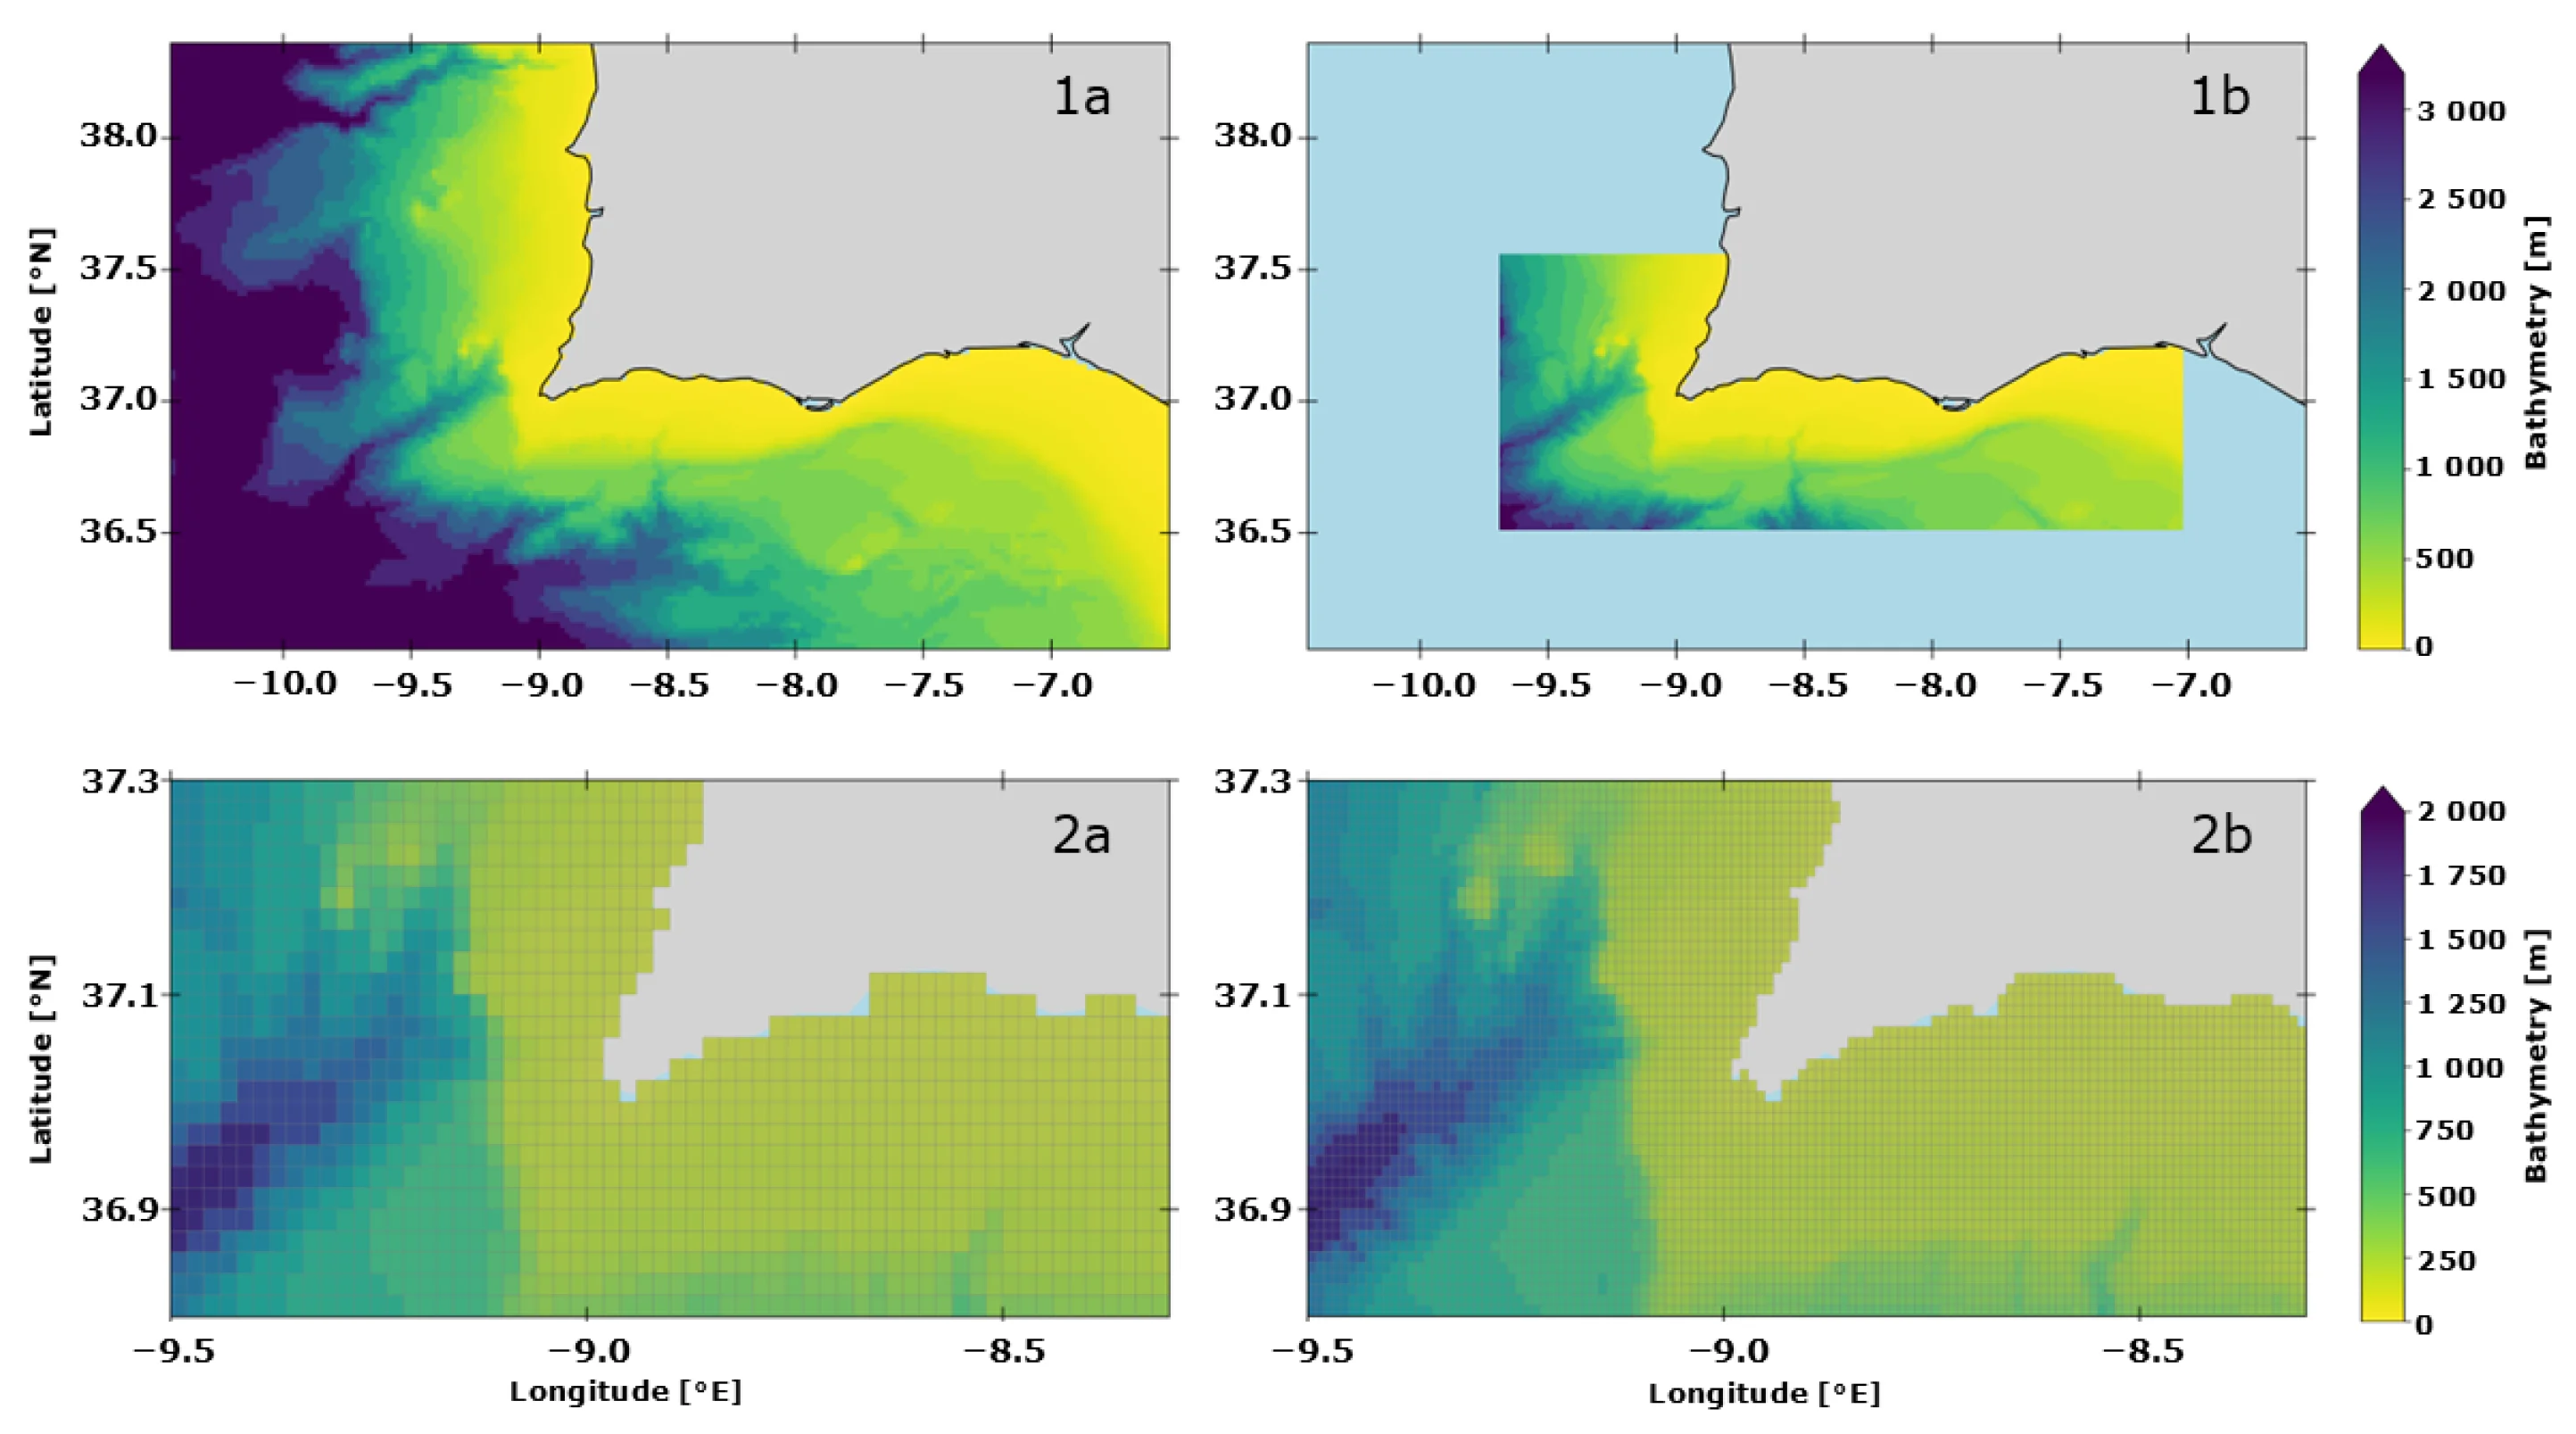
\includegraphics[width=16.0 cm]{figures/fig2.1.png}
    \caption{Spatial domains of the Algarve operational model (SOMA) used in this study. Panels (\textbf{1a}, \textbf{1b}) display the full extent of the SOMA Level 1 and Level 2 grids, respectively. Panels (\textbf{2a}, \textbf{2b}) present a zoomed-in view of the region surrounding Cape St. Vincent, located at the southwestern tip of the Algarve, to highlight the difference in spatial resolution between the two grid levels.}
    \label{fig:batim_2.1}
\end{figure}

In the operational cycle of SOMA, Level 0 is used exclusively to generate tidal boundary conditions and does not produce valid forecast data. In contrast, Levels 1 and 2 provide four-day forecasts of SSH, as well as three-dimensional fields of temperature, salinity, and ocean currents. A noteworthy aspect, as highlighted in \parencite{mendonca2023smscoastal}, is SOMA's operational strategy of performing weekly restart simulations based on CMEMS boundary conditions. This operational configuration serves to update the initial conditions for each new forecast cycle and is explored in the OSSE system implementation for SOMA, as detailed in the following section.

\subsection{SOMA OSSE System Design} \label{subsec:ossedesign_somaosse}
\subsubsection{Nature-Run and Free-Run Configurations}
\hypertarget{subsec:ossedesign_nrfr}{}

As outlined in the objectives of this study, the OSSE system was specifically developed to operate using SOMA as the background model. Given this premise, the ocean-model component of the OSSE is not a variable under investigation but is rather assumed to be a fixed and fully operational system. However, the experiment requires simulation of two different ocean states: one representing the true state (the NR) and another emulating a typical forecast scenario (the FM). In this work, the distinction between NR and FM was achieved by applying the fraternal twins approach, which resulted in using two different configurations of SOMA.

To represent the NR, this study relied on the existing SOMA forecast database for the year 2023. In other words, the key features of the NR within the OSSE system include the use of the Level 2 grid characterized by a horizontal resolution of 1 km and the incorporation of weekly restart cycles based on CMEMS boundary conditions. In contrast, configuring the FM required the introduction of controlled perturbations to SOMA to ensure that its evolution would diverge sufficiently from that of the NR while remaining physically realistic. The FM was initialized with the same initial conditions used for the NR at the start of 2023, as generated by a restart simulation. However, the main structural change involved modifying the Level 2 grid, which was applied over the area illustrated in \bCref{fig:batim_2.1}, panel 1b, by reducing its resolution to 2 km, thereby matching the coarser Level 1 grid shown in panel 2a of the same figure. Furthermore, unlike the NR, the FM was executed continuously throughout 2023 without any weekly updates from CMEMS. As a result, this configuration is referred to as the Free Run (FR), and it constitutes the second instance of SOMA used for comparison against the NR according to the metrics described in Section~\ref{sec:ossedesign_appxA}.

\subsubsection{Data-Assimilation System}
The next fundamental component of the OSSE is the DA system, responsible for incorporating synthetic observations into the FR. The assimilation algorithm employed was based on the formulation presented in \textcite{counillon2023framework}. Modifications were made to ensure compatibility with the SOMA model grid and to enable the reading of synthetic observation data as input, as described in the item \hyperlink{subsec:ossedesign_synthetic}{\textbf{Synthetic Observations and the Reference OSE}} of this Section.

The ensemble used to estimate the background error covariance in the EnOI scheme was sampled from the SOMA FR integration, the same model that was updated by the synthetic observations. Throughout the full-year integration of 2023, model states were extracted at regular intervals, specifically at a rate of one state every 25 h, in order to avoid tidal aliasing; the resulting total comprised 354 ensemble members. This sampling strategy was designed to capture the system's natural variability across the range of oceanographic conditions of the implemented region. Given the strong seasonal behaviour of the Algarve's circulation, as discussed in Section \ref{sec:ossedesign_algarve}, the ensemble was considered sufficient to represent background error structures.

In this implementation, the weighting coefficient $\alpha$, which regulates the balance between the background ensemble variance and the observation error covariance in the analysis update (Section \ref{sec:ossedesign_appxB}), was set to the default value of $1.0$. This choice effectively gives greater weight to the observations. While previous sensitivity studies have shown that smaller values of $\alpha$ may reduce spurious noise at the cost of weaker updates \parencite{counillon2009high}, higher values improve the initial agreement with observations, albeit at the expense of forecast accuracy at longer lead times. Because the present study was dedicated to the development and demonstration of the OSSE framework rather than to parameter optimization, a sensitivity analysis was not performed here. This represents a limitation of the current implementation; therefore, a systematic evaluation of $\alpha$ will be addressed in a future study.

In DA systems, localization functions are commonly employed to reduce the impact of spurious long-range correlations, which are common in ensemble-based DA methods due to finite ensemble size \parencite{carrassi2018data}. Due to this, the localization algorithm implemented in the adopted EnOI scheme was used, considering the Gaspari--Cohn correlation function \parencite{gaspari1999construction}. It is a quasi-Gaussian function that becomes exactly zero beyond a certain distance (compact support) but decreases the correlation values gradually and continuously as the distance increases (smooth tapering). This ensures that the transition from full to zero correlation is smooth, which avoids the introduction of artificial discontinuities into the assimilation process and is effective in addressing the correlation decay issue. The localization radius was set to 10 grid cells, which corresponds to a physical scale of 20 km in the SOMA FR configuration.

\subsubsection{Synthetic Observations and the Reference OSE}
\hypertarget{subsec:ossedesign_synthetic}{}

The final component of the OSSE system is the process of extracting synthetic observations from the NR integration. As previously described, those observations are not actual measurements obtained from external instruments. Instead, they are values picked from a field of SOMA via extraction directly from the model's state vector during the NR simulation. These values are then treated as if they were observational data and assimilated into the FR. To achieve this, a specific procedure was implemented to extract data from the NR outputs at predefined spatial and temporal locations chosen to mimic the structure of a realistic observation network.

Although the assimilation update is applied to the full three-dimensional model domain, the current implementation of the DA system in SOMA was restricted to surface observations. Extending the system to incorporate subsurface data remains a technical challenge due to the complexities of vertical localization and observation operator design. Therefore, it was left for future development. Within this constraint, the experiments employed a univariate DA approach in which SST observations were assimilated to update the complete 3D temperature structure of the model. In other words, temperature was the only variable included in the model state vector of the DA system. This variable has a central role in regulating key oceanic processes such as vertical mixing, stratification, and density-driven circulation. Thus, even when it is assimilated as a single variable, it can exert a wider influence on the modelled ocean state, indirectly improving other variables through the dynamical balances represented in SOMA.

In this context, the synthetic SST observations were extracted from the surface layer of SOMA's Level 2 grid in the NR solution. A hierarchical random strategy based on a spatial sampling approach was implemented. In this approach, the horizontal domain was divided into a regular grid of subareas, each one defined by a fixed number of model grid cells forming a square. Within each subarea, a single observation point was randomly selected using the \verb|randint| function from Python's (version 3.12) \verb|random| module, which generates a pseudo-random integer corresponding to a specific grid cell location. This procedure was applied iteratively across the entire layer, ensuring an irregular but homogeneously distributed set of observations. Consequently, the density of observations depends on the size of the subareas: smaller subareas result in a larger number of observation points, while larger subareas yield fewer but more sparsely distributed observations.

It is crucial to emphasize that for an OSSE system to be reliable, the errors associated with the synthetic observations should not be derived from the NR itself. Instead, they should realistically replicate the kinds of uncertainties present in actual observational systems \parencite{halliwell2014Rigorous}. This requires additional assumptions, as synthetic observations do not originate from physical instruments and thus lack the natural noise introduced by sensors, platforms, or environmental conditions. To guide the estimation of the errors and establish a realistic reference for comparison, two operational satellite-based products covering the SOMA region in 2023 were considered.

\begin{itemize}
	\item CMEMS SST NRT ODYSSEA L4 Product \parencite{eucmems2019ho}: an operational monitoring product providing near-real-time (NRT) SST fields. Updated daily, it is optimized for operational forecasting and rapid environmental monitoring. This product has a finer spatial resolution of $0.02^{\circ}$ and is designed to capture short-term variability. 
	\item CMEMS SST Reprocessed L4 Product \parencite{eucmems2019qa}: a historical, consistently reprocessed climate product that has been available since 1 January 1982. It offers high-quality SST fields produced with rigorous reanalysis methods and quality-control protocols. The product is intended for climate studies and long-term analyses, with a horizontal resolution of $0.05^{\circ}$.   
\end{itemize}

Both satellite products share similar characteristics, providing SST data along with the corresponding estimated observation error standard deviation. Using more than one dataset of the same type ensures that the OSSE system is evaluated under consistent conditions, so that the experiments are expected to produce comparable responses rather than to behave differently depending on the chosen dataset. In addition to their role in defining the OSSE observation errors, these products also served as the observational sources for the reference OSE system. For this purpose, the extraction of data points was restricted to the spatial extent of the NR domain (SOMA Level~2). Within this area, observations were selected using the same pseudo-random sampling strategy previously described for the synthetic data, and for each point, the error value provided by the satellite product was directly applied in the assimilation process of the OSE experiments.

In the OSSE experiments, the procedure to define the observation errors began with identification of the base error value at each observation point from the corresponding satellite product used in the comparative OSE experiment. In other words, if the OSSE configuration was designed to be evaluated against an OSE using the NRT ODYSSEA dataset, then the base error at each synthetic observation point in the OSSE was initially taken from the same spatial location in that product. However, direct assignment of these values would result in an unrealistic equivalence of errors between the systems, contradicting the principle that synthetic observations must emulate, not replicate, real observational noise. To overcome this limitation and preserve the integrity of the OSSE system, a spatially correlated random perturbation field was applied to the base error values. This field was generated using a FORTRAN algorithm based on the methodology described in Appendix E of \parencite{evensen2003ensemble}. The output is a two-dimensional pseudo-random field with horizontal correlation that smoothly varies the values across the model grid to ensure that neighbouring points are not perturbed independently.

Following the exposed methodology, each OSE and OSSE experiment consisted of the assimilation of a single set of surface observations into the FR. The experimental  design involved a structured sequence of steps. First, a set of potential observation points was extracted from the NR grid using the pseudo-random spatial sampling procedure described earlier. From this initial set, a subset was randomly selected, also using the \verb|random| module from Python, to define the number of observations to be assimilated. This reduction process was repeated multiple times using the same base set to generate different observation scenarios containing 10, 50, 100, 200, and 500 data points. Each observation in these sets was associated with an error estimate derived from the corresponding satellite product and perturbed using the spatially correlated random field previously described. Importantly, a different perturbation field was applied to each observation set, ensuring independent spatial patterns of error for each experiment. This behaviour is possible because the FORTRAN program used for generating these fields initializes the random number generator with a seed derived from the system clock, which ensures that a distinct perturbation is produced at each execution over the same model grid. This experimental design is summarized in \bCref{tab:exps_2.1}.

\section{Results and Discussion} \label{sec:ossedesign_results}

This section presents the outcomes of the experiments conducted with the OSSE system configured for the SOMA model. The results are structured into two parts: the first subsection focuses on the analysis of FR integration, which served as the forecast model in the OSSE. It includes a comparison of its temperature fields with the NR, along with an assessment of variability among ensemble members and spatial correlation. The second subsection addresses the core objective of this work: the comparative evaluation of the OSSE and OSE experiments using the various observational scenarios described in the previous section.

\begin{table}[H]
	\centering
	\caption{Summary of the OSE and OSSE experiments. Each experiment is defined by the number of surface observation points assimilated (column \textbf{Number of Points}), the data source from which SST values were extracted (\textbf{Data Source}), and the method used to obtain or estimate the observation errors (\textbf{Observation Error}).}
	\label{tab:exps_2.1}
	\footnotesize
	\begin{tabular}{ccccc}
		\toprule
		\textbf{Experiment}	& \textbf{\shortstack{Number of\\Points}} & \textbf{\shortstack{Data\\Source}} & \multicolumn{2}{c}{\textbf{\shortstack{Observation\\Error}}}\\
		\midrule
		OSE\textsubscript{1} & 10 & \multirow{5}{*}{\shortstack{CMEMS NRT\\ODYSSEA}} & \multicolumn{2}{c}{\multirow{5}{*}{from data source}}\\
		OSE\textsubscript{2} & 50 & & \\
		OSE\textsubscript{3} & 100 & & \\
		OSE\textsubscript{4} & 200 & & \\
		OSE\textsubscript{5} & 500 & & \\
		\midrule
		OSE\textsubscript{6} & 10 & \multirow{5}{*}{\shortstack{CMEMS\\Reprocessed}} & \multicolumn{2}{c}{\multirow{5}{*}{from data source}}\\
		OSE\textsubscript{7} & 50 & & \\
		OSE\textsubscript{8} & 100 & & \\
		OSE\textsubscript{9} & 200 & & \\
		OSE\textsubscript{10} & 500 & & \\
		\midrule
		OSSE\textsubscript{1} & 10 & \multirow{5}{*}{\shortstack{SOMA\\Nature Run}} & \multirow{5}{*}{NRT\_ODYSSEA $\times$} & random\_field\textsubscript{1}\\
		OSSE\textsubscript{2} & 50 & & & random\_field\textsubscript{2}\\
		OSSE\textsubscript{3} & 100 & & & random\_field\textsubscript{3}\\
		OSSE\textsubscript{4} & 200 & & & random\_field\textsubscript{4}\\
		OSSE\textsubscript{5} & 500 & & & random\_field\textsubscript{5}\\
		\midrule
		OSSE\textsubscript{6} & 10 & \multirow{5}{*}{\shortstack{SOMA\\Nature Run}} & \multirow{5}{*}{Reprocessed $\times$} & random\_field\textsubscript{6}\\
		OSSE\textsubscript{7} & 50 & & & random\_field\textsubscript{7}\\
		OSSE\textsubscript{8} & 100 & & & random\_field\textsubscript{8}\\
		OSSE\textsubscript{9} & 200 & & & random\_field\textsubscript{9}\\
		OSSE\textsubscript{10} & 500 & & & random\_field\textsubscript{10}\\
		\bottomrule
	\end{tabular}
\end{table}

\subsection{SOMA Free Run Integration}
The FR simulation was integrated continuously throughout the year 2023, following the configurations and conditions detailed in the item \hyperlink{subsec:ossedesign_nrfr}{\textbf{Nature-Run and Free-Run Configurations}} of Section \ref{subsec:ossedesign_somaosse}. Since SST is the common variable provided by both satellite products selected as observational sources in the reference OSE system, it was also adopted as the basis for assessing the performance of the FR against the NR. Accordingly, the annual evolution of the instantaneous spatial averages (as defined by \bCref{eq:cp2_avg}) and the corresponding RMSEs (\bCref{eq:cp2_rmse}) were computed over the Level~2 domain for both integrations, and the results are presented in the chart in \bCref{fig:sstavg_2.2}.

As shown in \bCref{fig:sstavg_2.2}, the NR and FR exhibit similar seasonal patterns, but their magnitudes vary throughout the year. The RMSE values fluctuate, with higher errors occurring during three distinct periods: early in the year (January-February), in mid-summer (July-August), and late in the year, as the cold season begins. The largest discrepancies align with the transitions between warm and cold seasons, suggesting that the differences between NR and FR are more pronounced during these periods. Despite these differences, the FR solution consistently followed the same seasonal trend as the NR solution did, reflecting a coherent thermal cycle over the year. In certain periods, particularly during spring and early autumn, the SST fields of both solutions were notably close, likely due to the constraint of the shared boundary conditions used in both simulations. Even then, this alignment is seen as a positive result because it reinforces the realism of the FR, while it still represents a degraded solution.

\begin{figure}[H]
	\centering
	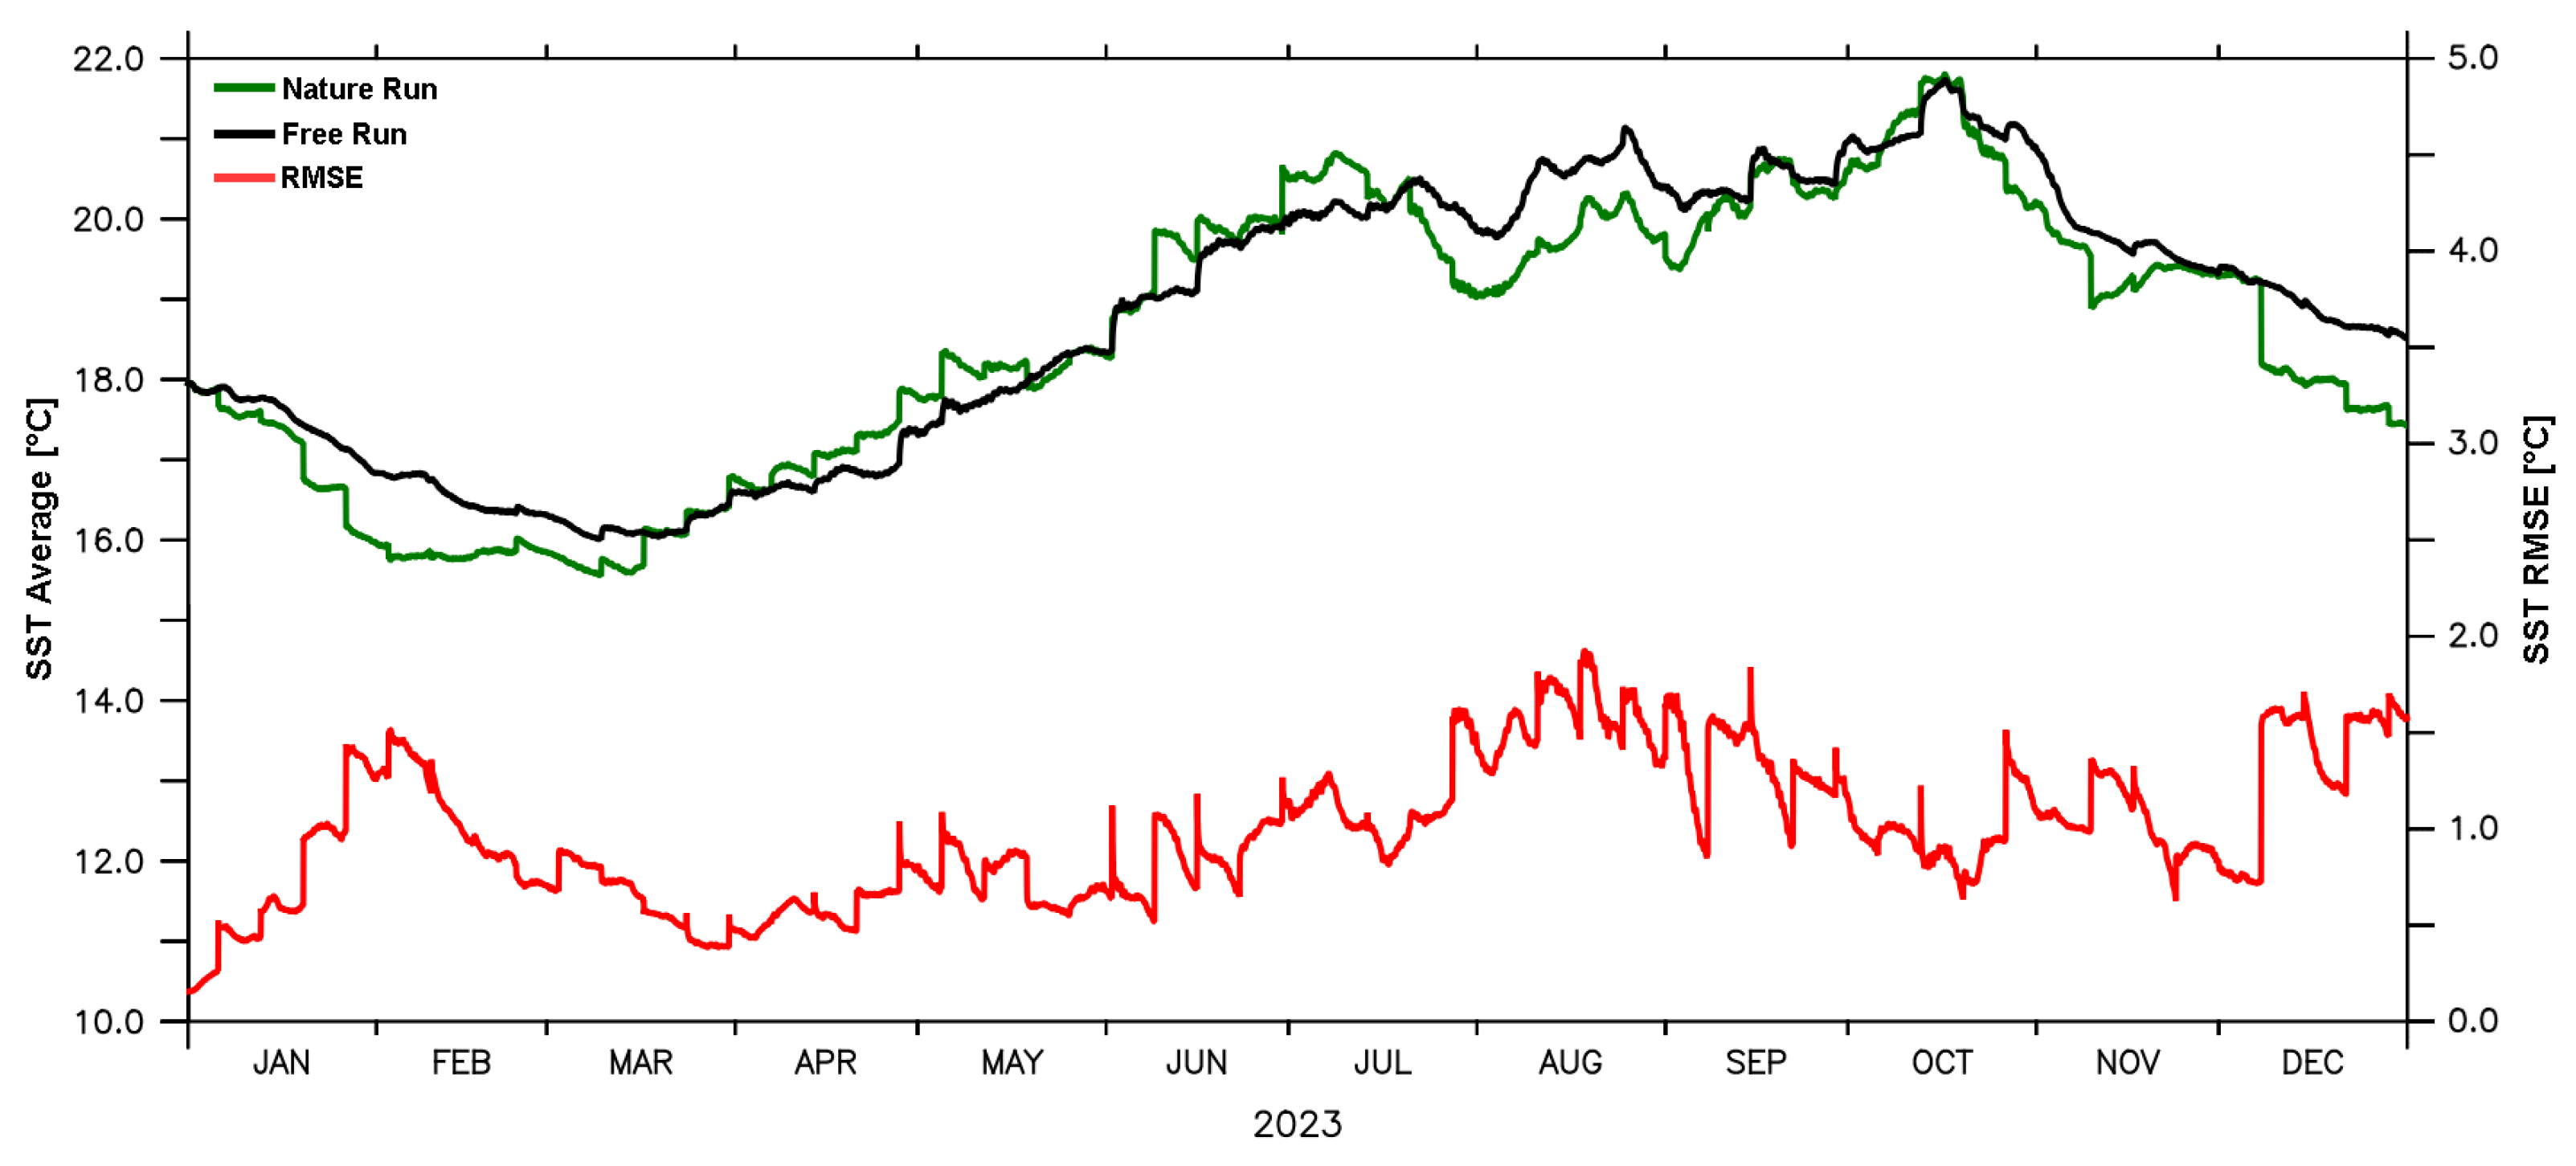
\includegraphics[width=16.0 cm]{figures/fig2.2.png}
	\caption{Comparison of sea surface temperature (SST) between the Nature Run (NR, green line) and the Free Run (FR, black line) over the year 2023. The root mean square error (RMSE) between the temperature fields is shown by the red line, with its scale indicated on the secondary \emph{y}-axis (right)}
	\label{fig:sstavg_2.2}
\end{figure}

A closer inspection of the NR SST curve reveals more pronounced discontinuities, visible as sharp jumps in temperature that are not present in the FR. These abrupt changes are a clear visual indication of the weekly restart simulations implemented in the NR, which force SOMA state variables directly from the updated data of the CMEMS Global solution product. This approach is inherited from the standard SOMA operational forecast framework. Since such updates were deliberately excluded from the FR solution to simulate an unconstrained forecast, these differences further highlight the structural divergence between the two integrations.

It can be inferred that the most significant discrepancies between NR and FR align with the moments of the weekly adjustments, highlighting their influence on the thermal evolution of the NR. This behaviour is particularly evident in the first months of 2023, where the NR solution exhibits a sharper decline in SST compared to the FR in late January and the beginning of February. The influence of the restart mechanism forces the solution to more closely follow the cooling patterns present in the CMEMS data. In contrast, the FR retains more thermal inertia and cools more gradually. At the end of the cold season, the FR lags behind the NR, which begins to recover earlier in response to the updated forcing fields. This example illustrates how the absence of regular external updates in the FR leads to smoother but slower thermal transitions, further supporting the appropriateness of the FR's role as a realistically imperfect forecast scenario within the OSSE framework.

While it is reassuring that the FR solution remained stable and physically consistent, it is nevertheless desirable for it to diverge as much as possible from the NR solution. The larger the discrepancies between them, the greater the system's sensitivity to the observation inputs. This increased sensitivity makes it easier to quantify the added value of the synthetic observations. With this in mind, a specific time frame was selected for conducting both the OSSE and OSE experiments. The selection was guided by the temporal evolution of the RMSE (red curve in \bCref{fig:sstavg_2.2}), which pointed to early February as one of the periods of maximum disagreement between NR and FR. At the same time, it was necessary to consider the availability and quality of satellite observations, which are often affected by cloud cover. Consequently, February 3rd was identified as an optimal date, at it balanced a high RMSE with favourable observational conditions.

Before the observation experiments could begin, an initial assessment of the correlation structure among the ensemble variables in the FR was performed. Given that SST is the primary variable updated through the assimilation process in this system, it was important to examine how it correlates with other physical fields across the model domain. To this end, correlation coefficients were computed between the SST time series at a fixed surface grid cell and the time series of all other variables at each cell within the same horizontal layer. The time series were derived from the FR ensemble members; that is, there was one value for each 25 h period of 2023. Two reference points were selected for this analysis: one located along the southern coast (36.95$^\circ$ N, 7.73$^\circ$ W), an area influenced by the countercurrent system, and another on the western coast (37.29$^\circ$ N, 9.09$^\circ$ W), where coastal upwelling plays a dominant role. The resulting correlation maps, presented in \textbf{Figures}~\bref{fig:corrS_2.3} and~\bref{fig:corrW_2.4}, provide valuable insight into the spatial coherence and dynamical relationships represented by the ensemble.

No correlation plots for SST and SSH are presented here, as the analysis did not reveal any significant relationship between these variables in the FR ensemble. \bCref{fig:corrS_2.3} depicts the correlation maps for the southern reference point. Panels 1.A and 2.A show the correlation between SST and salinity at the surface and at a depth of 100 m, respectively, while panels 1.B and 2.B depict the correlation between SST and horizontal currents at the two same depths. A clear negative correlation is observed between SST and salinity in the ensemble, and this becomes more pronounced with depth. This result indicates that, within the variability represented by the ensemble, colder waters at the surface of the south coast tend to be associated with higher salinity in this region, potentially reflecting the vertical mixing process simulated by the model. In contrast, the correlations between SST and current velocity are weakly positive near the surface and become even less significant at greater depths.

\begin{figure}[H]
	\centering
    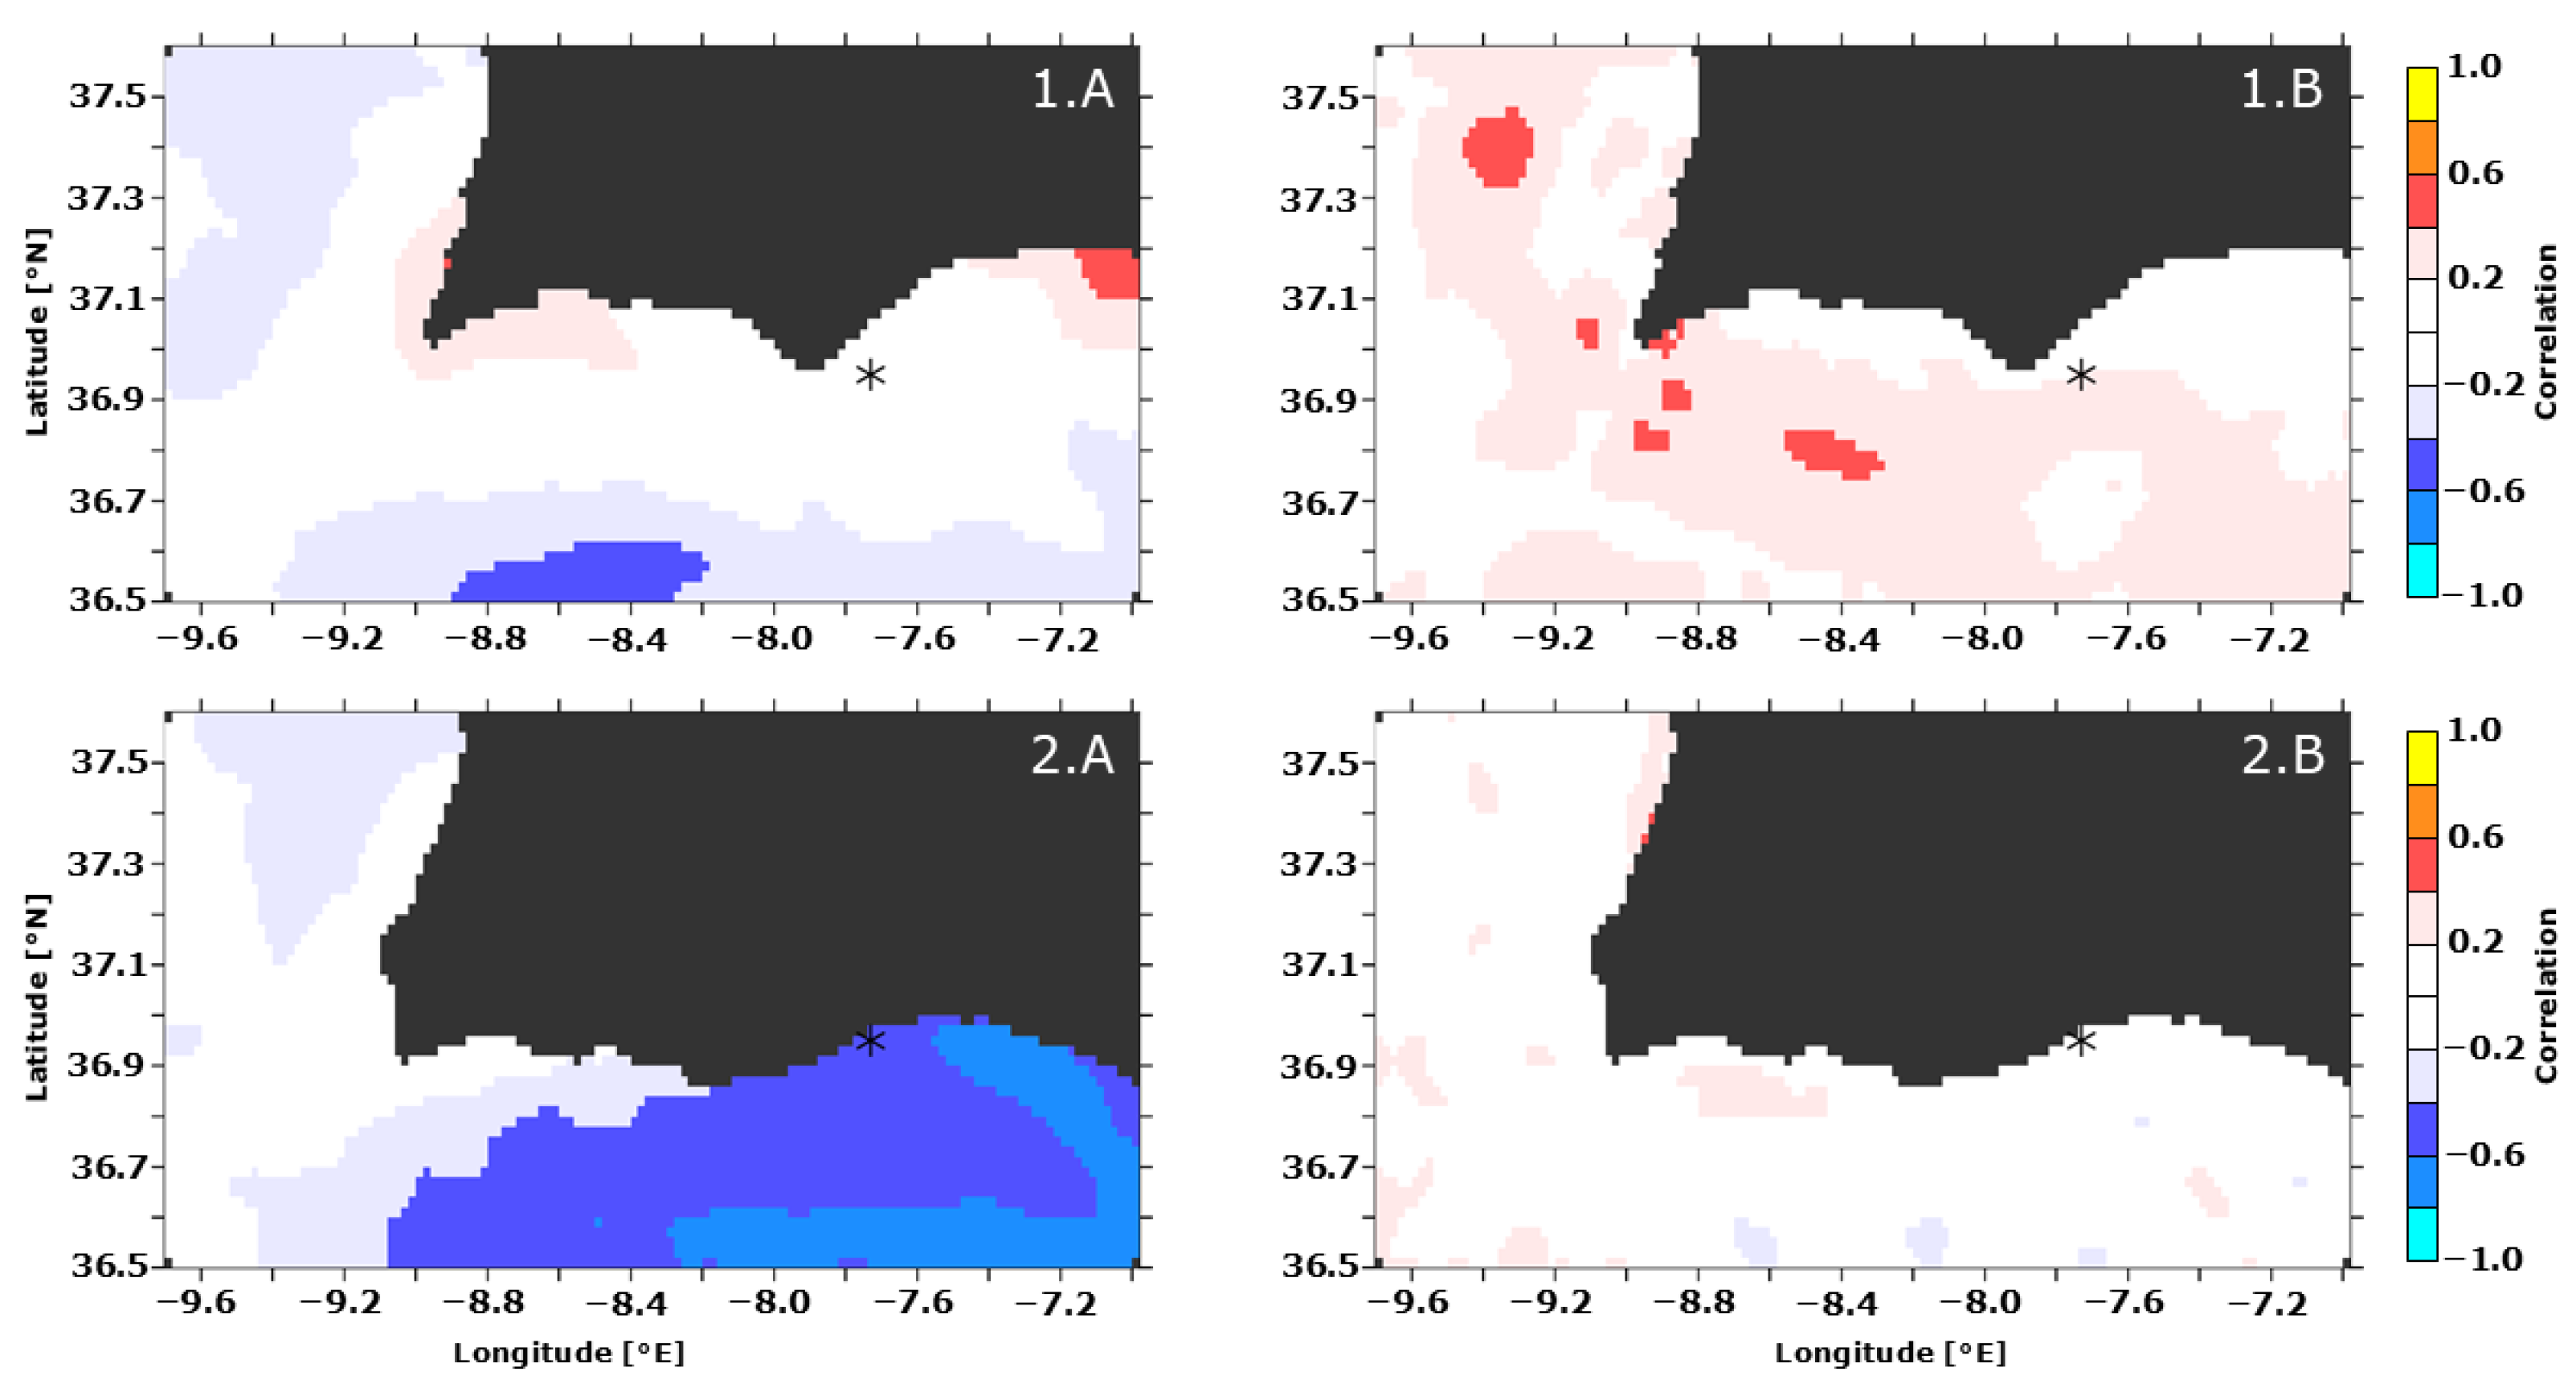
\includegraphics[width=16cm]{figures/fig2.3.png}
    \caption{Correlation maps computed using a reference point on the surface (asterisk on the maps, 36.95$^\circ$ N, 7.73$^\circ$ W). The correlation was calculated over time across all FR ensemble members, relating the surface temperature at this fixed point to salinity and current fields in the rest of the model grid. Maps (\textbf{1.A},\textbf{1.B}) show the correlations at the surface for salinity and currents, respectively. Maps~(\textbf{2.A},\textbf{2.B}) depict the same properties at a depth of 100 m.}
    \label{fig:corrS_2.3}
\end{figure}

\begin{figure}[H]
	\centering
	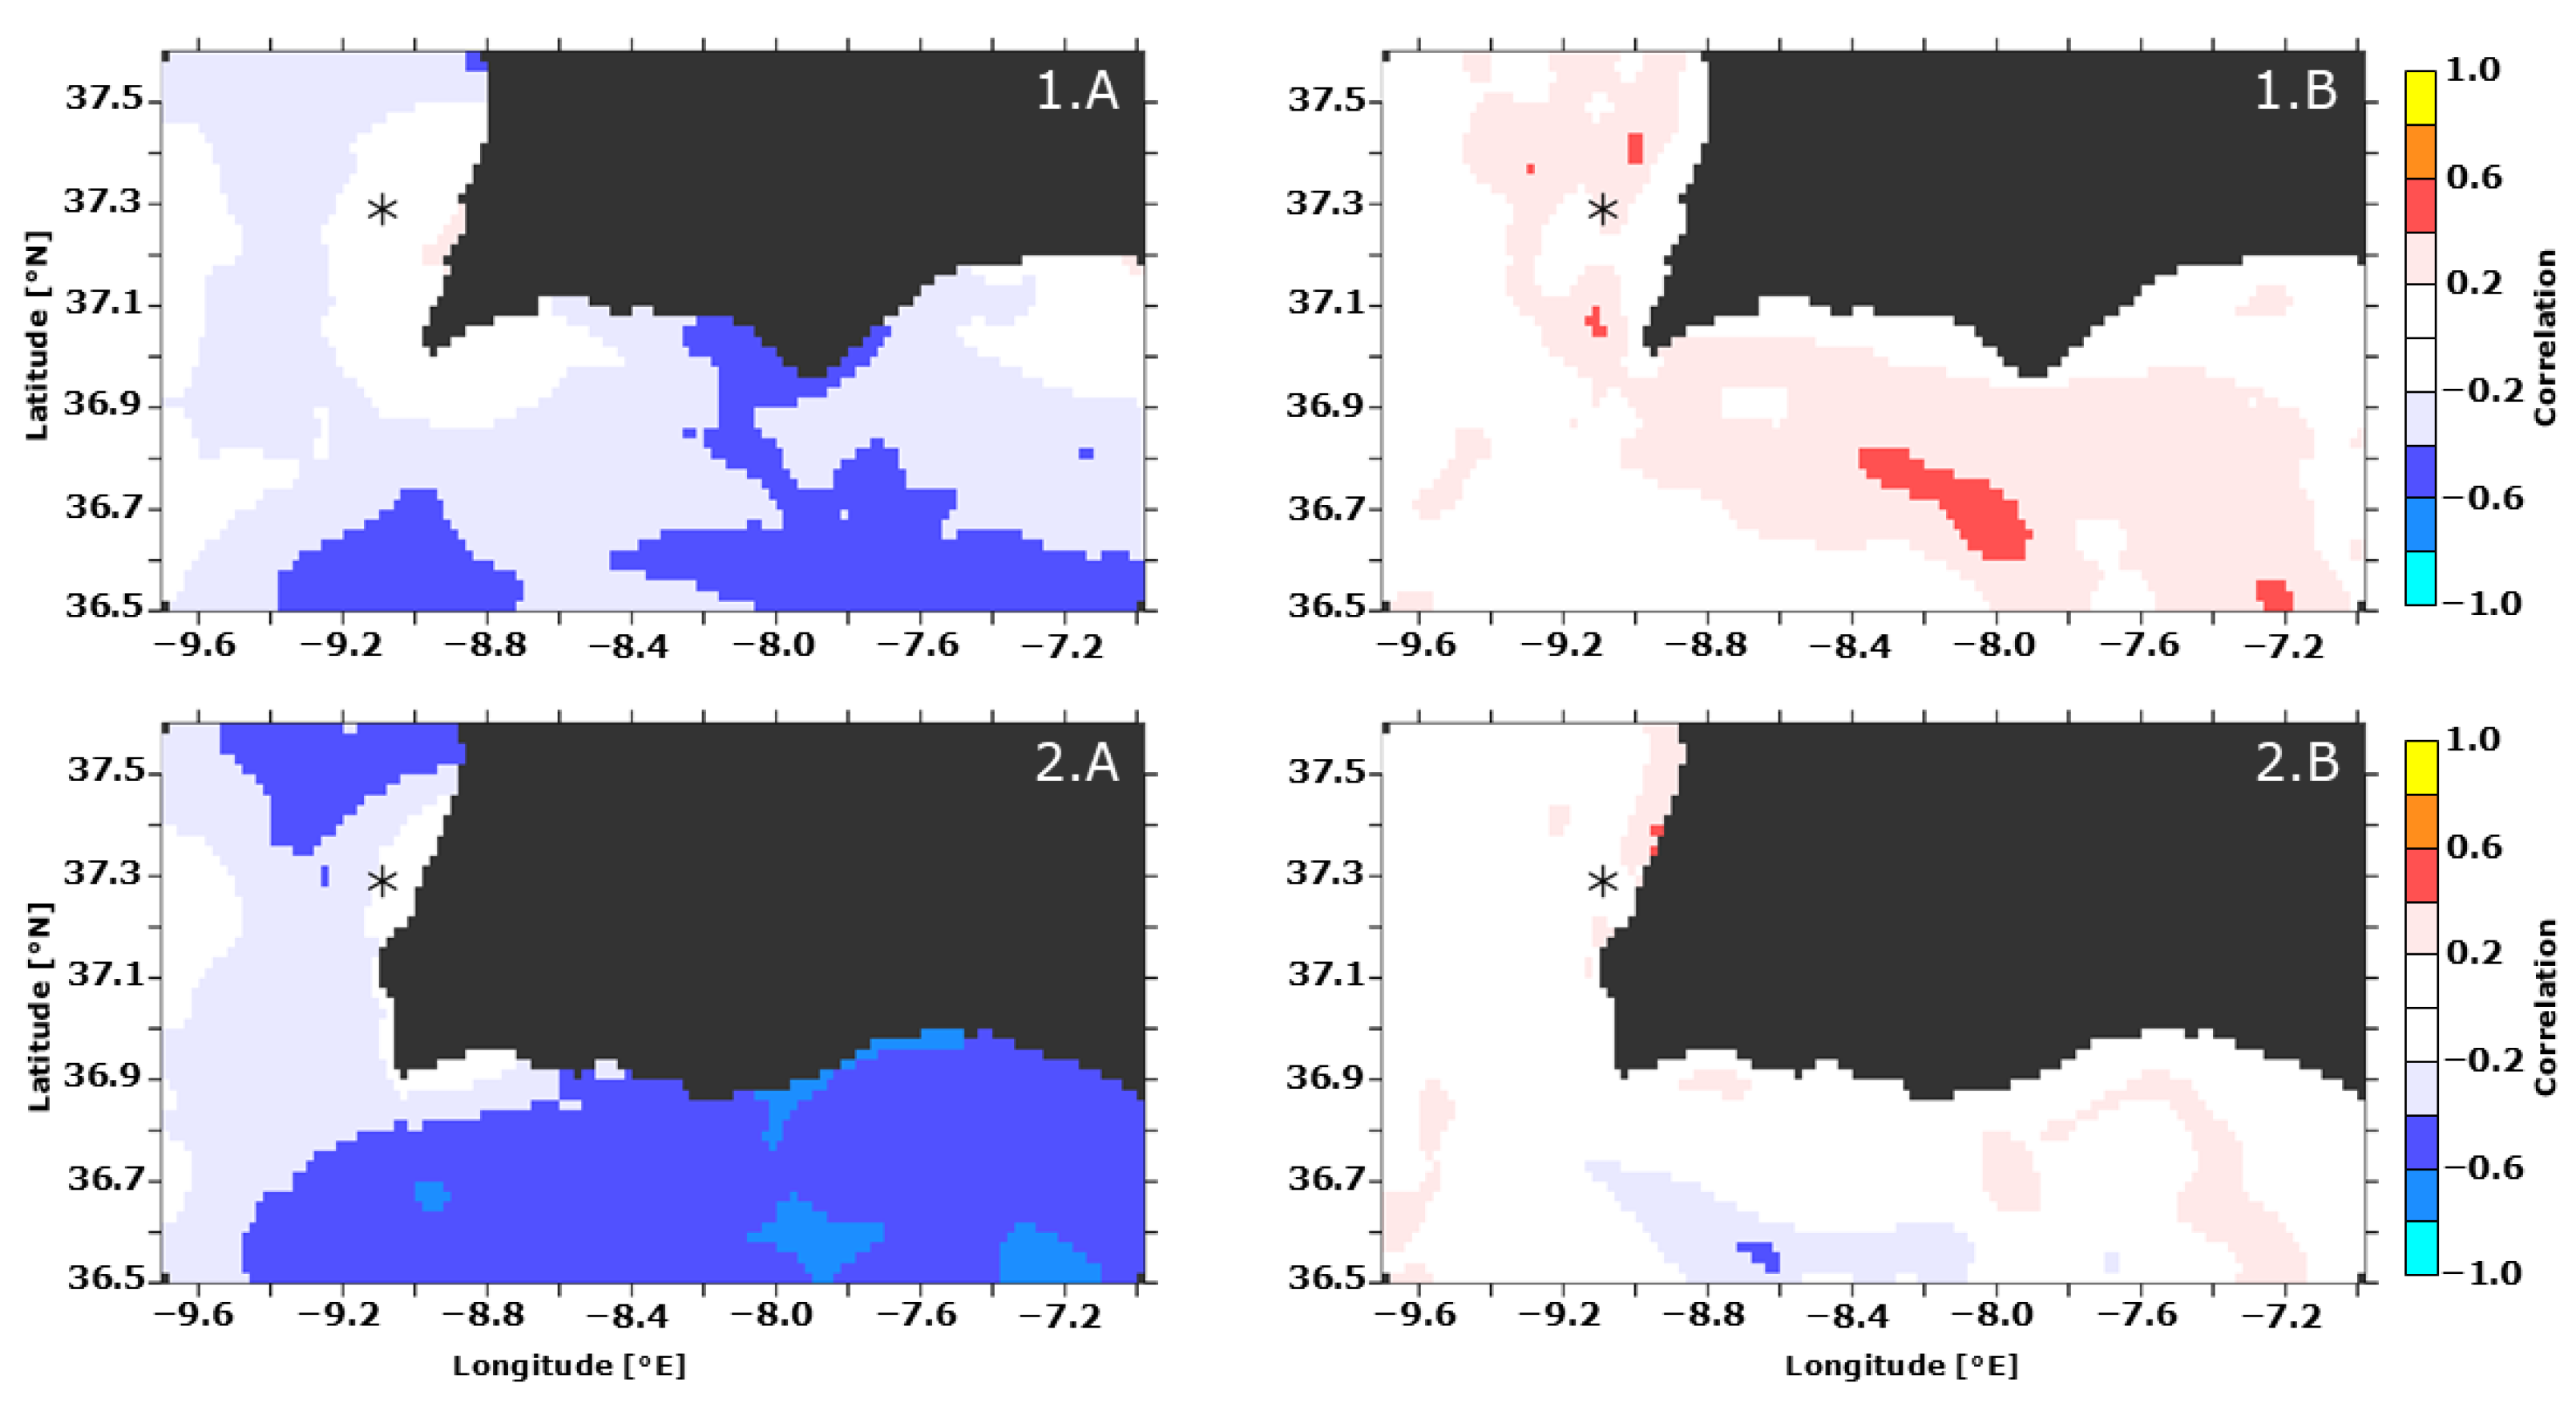
\includegraphics[width=16cm]{figures/fig2.4.png}
	\caption{Correlation maps computed using a reference point on the surface (asterisk on the maps, 37.29$^\circ$ N, 9.09$^\circ$ W) on the western coast of the domain. The correlation was calculated over time across all FR ensemble members, relating the surface temperature at this fixed point to salinity and current fields in the rest of the model grid, following the same methodology as in \bCref{fig:corrS_2.3}. Maps (\textbf{1.A},\textbf{1.B}) show the correlation at the surface for salinity and currents, respectively, while Maps (\textbf{2.A},\textbf{2.B}) depict the same properties at a depth of 100 m.}
	\label{fig:corrW_2.4}
\end{figure}

\newpage
A similar pattern is observed in the maps shown in \bCref{fig:corrW_2.4}, which correspond to the western reference point influenced by upwelling. Again, panels 1.A and 2.A show the correlation with salinity at the surface and 100 m, while 1.B and 2.B refer to the correlation with horizontal currents. As in the southern region, SST is negatively correlated with salinity in the ensemble, and this correlation intensifies with depth. The relationship with currents shows a limited positive correlation near the surface that diminishes with depth, indicating that there is only a modest association between thermal variability and current patterns within the ensemble in this area as well.

Given the consistent negative correlation patterns between SST and salinity observed in \textbf{Figures}~\bref{fig:corrS_2.3} and~\bref{fig:corrW_2.4}, a vertical profile analysis was conducted to further investigate this relationship throughout the water column. Using the same two reference locations, the correlation  between the surface SST and salinity values was computed at increasing depths at each respective point. Hence, for each spot, the correlation was computed over time across all ensemble members and repeated for all vertical salinity levels in the model. The results (\bCref{fig:corrz_2.5}) reveal a clear intensification of the negative correlation with depth. The red curve represents the profile for the southern coast reference point, while the blue curve corresponds to the western location. In both cases, the strength of the inverse relationship increases steadily with distance below the surface, confirming that the inverse relationship between temperature and salinity becomes more pronounced with depth in the ensemble.

The results presented in \textbf{Figures}~\bref{fig:corrS_2.3}--\bref{fig:corrz_2.5} suggest a negative correlation between SST and salinity within the FR ensemble that becomes particularly pronounced at greater depths. Given that the OSSE system is based on an EnOI data-assimilation scheme, such a statistical relationship could, in principle, be leveraged in a multivariate assimilation framework \parencite{counillon2009ensemble, turner2005assimilation}. This would allow SST observations to contribute indirectly to salinity updates, potentially improving the model's representation of water mass properties and thermohaline structure. Such an approach also carries practical implications for the design of observing systems, as exploiting multivariate updates from SST could lessen the reliance on dedicated salinity measurements and thereby enable the deployment of lower-cost observing technologies and more extensive large-scale monitoring networks.

Although the ensemble reveals a statistical relationship between SST and salinity, the physical basis of this negative correlation remains uncertain. Specifically, in the southern region of the domain, a positive correlation between SST and salinity was initially anticipated, considering the influence of easterly winds that occur offshore of the south coast. These winds transport warm, saline Mediterranean waters toward the Algarve shelf and often alternate with westerly winds along the coastline (Section~\ref{sec:ossedesign_algarve}). The dynamics of these alternating wind regimes and their impact on surface and subsurface water properties may not be fully captured by the FR ensemble, especially if its sampling fails to represent the full range of seasonal variability. For this reason, and to preserve methodological clarity, the current implementation of the OSSE system was limited to temperature updates only, leaving multivariate approaches for future development once the underlying mechanisms are better understood.

\begin{figure}[H]
	\centering
	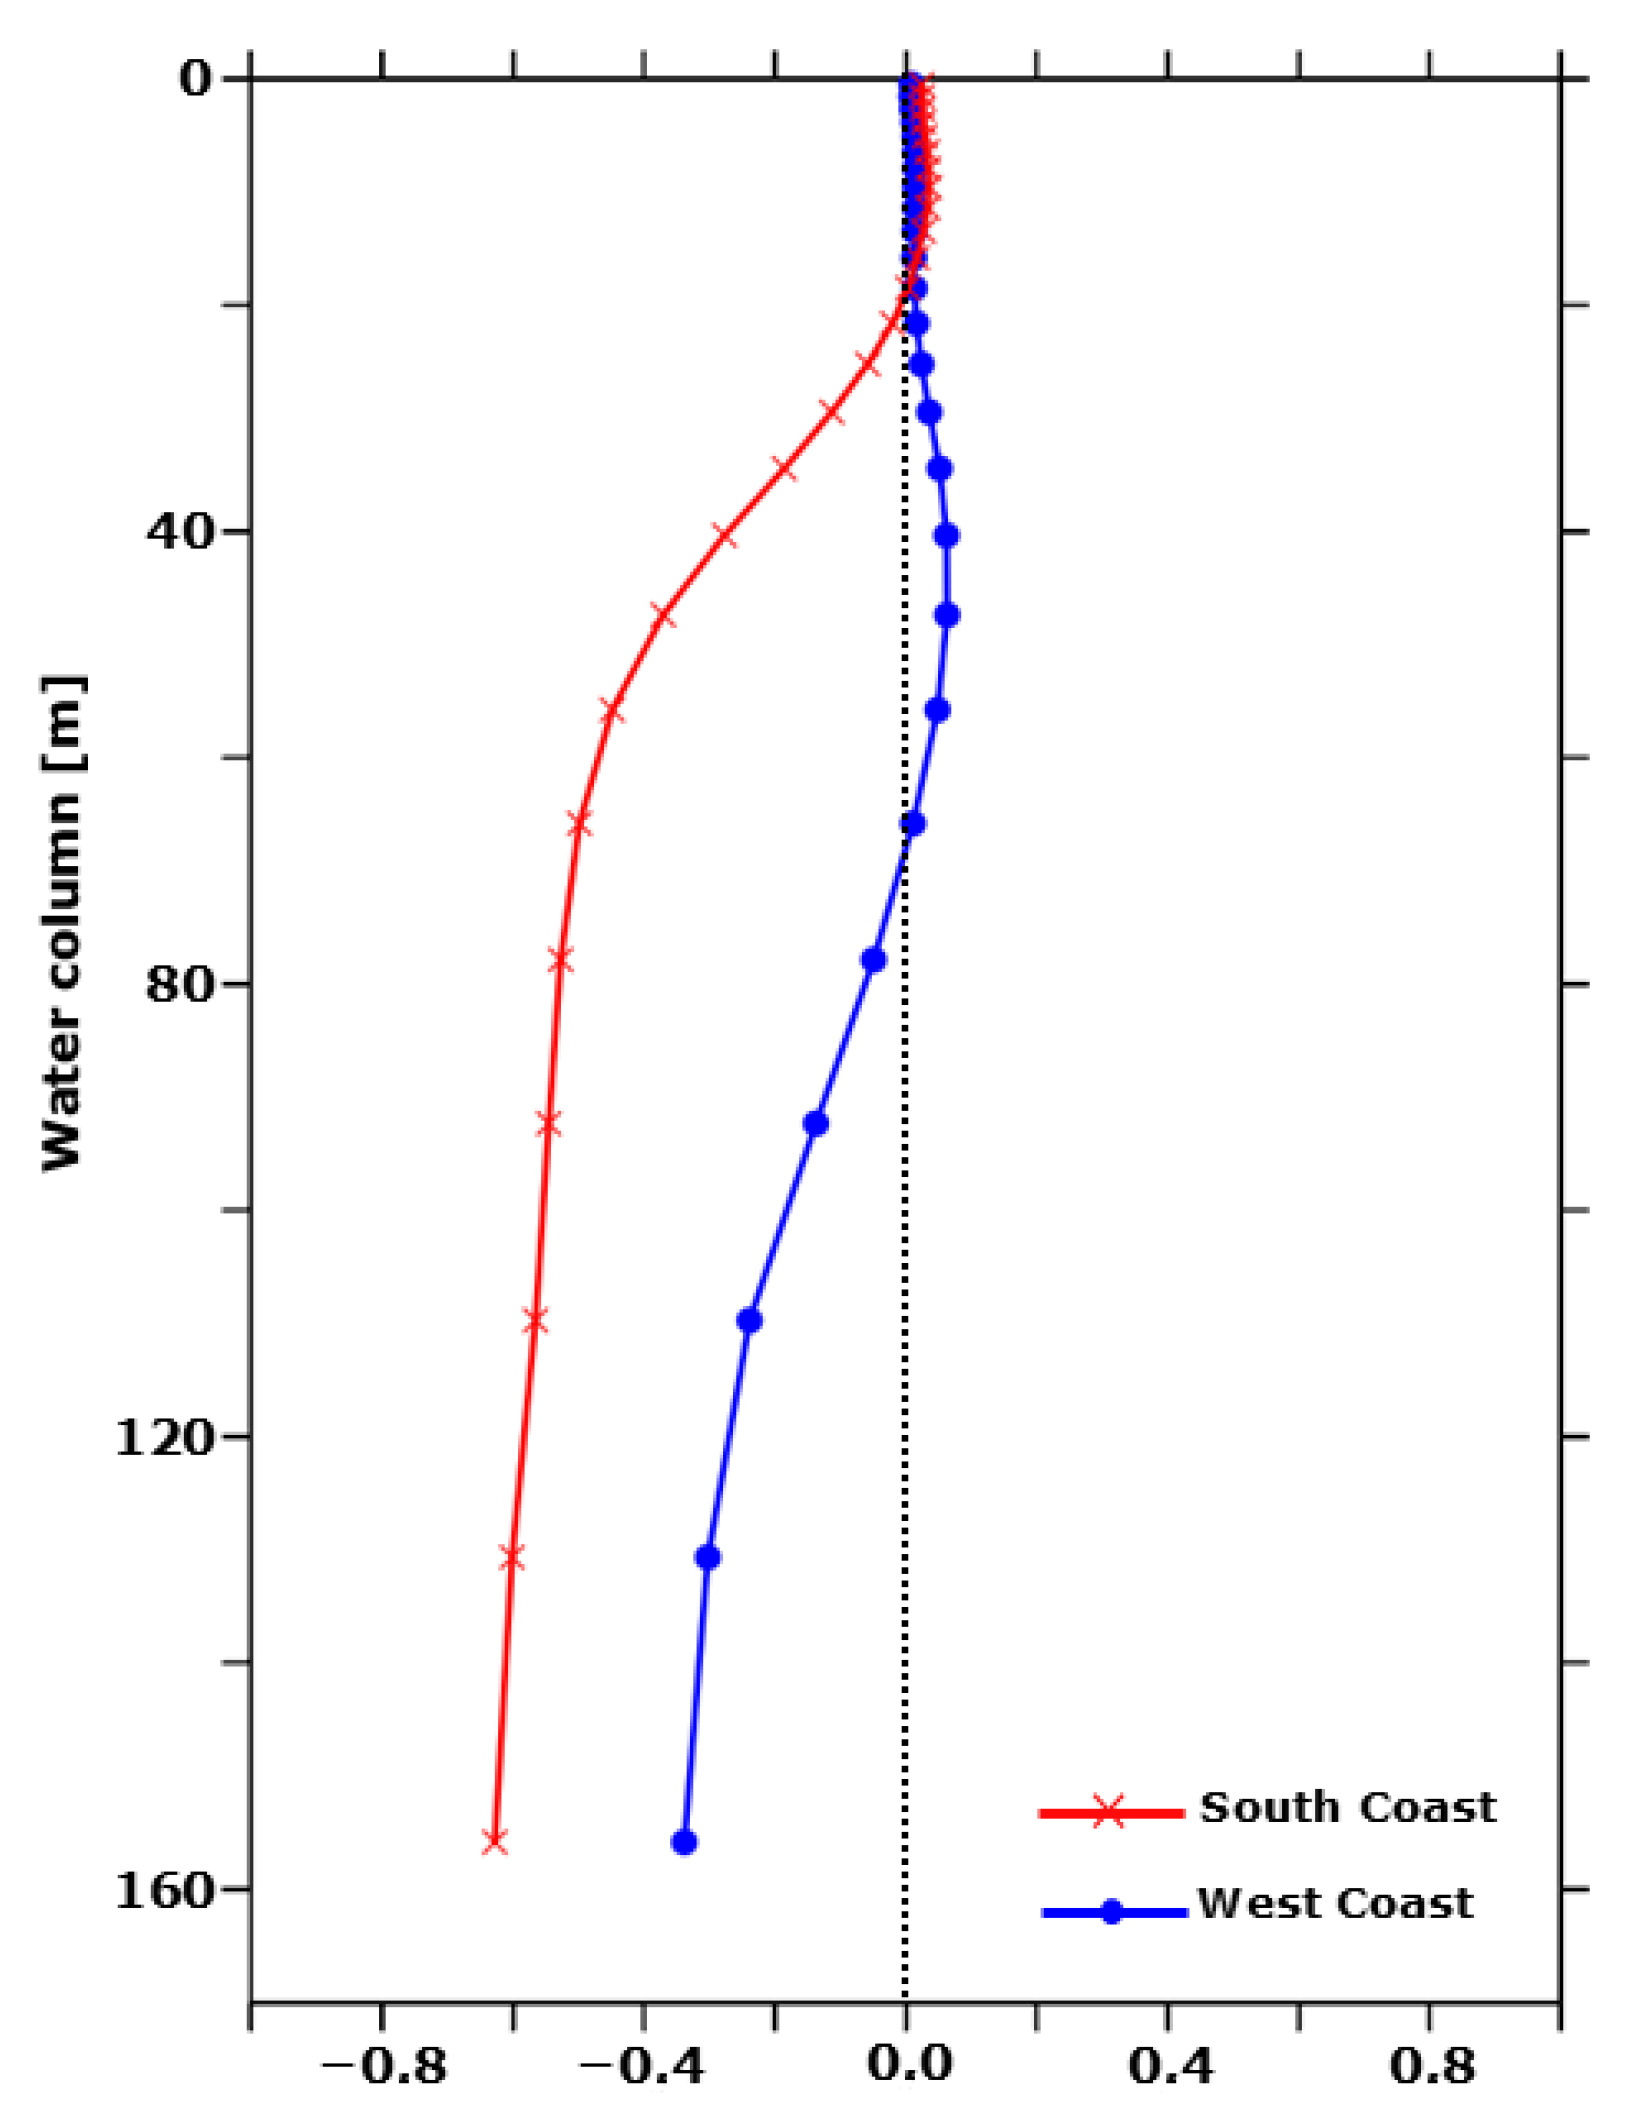
\includegraphics[width=9.0cm]{figures/fig2.5.png}
	\caption{Depth-dependent correlation between SST and salinity over time, calculated using the FR ensemble members. Each curve corresponds to a reference location within the model domain: the southern coast of Portugal (36.95$^\circ$ N, 7.73$^\circ$ W; red curve, same as \bCref{fig:corrS_2.3}) and the western coast (37.29$^\circ$ N, 9.09$^\circ$ W; blue curve, same as \bCref{fig:corrW_2.4}).}
	\label{fig:corrz_2.5}
\end{figure}

\subsection{SOMA OSSE System Assessment}

The performance and internal structure of the FR having been established, this section presents how it responded to the updates derived from the synthetic observations generated in the NR, as well as a comparative evaluation of the OSSE experiments and their corresponding OSE configurations. These analyses aimed to quantify the behaviour of the OSSE system to ensure that, when applied to assess new observation strategies, it would not systematically overestimate or underestimate their value.

Regarding the pseudo-random perturbation fields introduced in the item \hyperlink{subsec:ossedesign_synthetic}{\textbf{Synthetic Observations and the Reference OSE}} of \Cref{subsec:ossedesign_somaosse}, a horizontal decorrelation length had to be defined to determine the spatial scale over which values in a generated field remained correlated. This distance reflected the approximate range at which SST values in the L3 satellite products appear spatially coherent prior to their processing into the corresponding L4 gridded datasets. For this reason, a value of 25~km was selected, corresponding to 25 cells in the 1 km NR grid.

Knowing that 3 February 2023 was selected as the date for the updates, each experiment was subsequently integrated for an additional seven days to evaluate the temporal evolution of the forecast after the assimilation step. \bCref{fig:rmsenrt_2.6} presents the results of this post-assimilation period for the experiments based on the NRT ODYSSEA product. In the left-hand panel, the daily evolution of the SST RMSE is shown for each OSE experiment relative to the satellite observations, with the black curve representing the baseline FR error. The remaining curves correspond to OSEs using an increasing number of assimilated observation points, from 10 in OSE1 to 500 in OSE5, as listed in \bCref{tab:exps_2.1}. The right-hand panel displays the corresponding SST RMSE for the OSSE experiments, which assimilated synthetic observations and were evaluated against the NR. As expected, experiments using the Reprocessed product exhibited behaviour very similar to the behaviour of those that used the NRT ODYSSEA data. Therefore, the RMSE results from the Reprocessed-based experiments are presented in \Cref{sec:cp2_supp}


\begin{figure}[H]
    \centering
    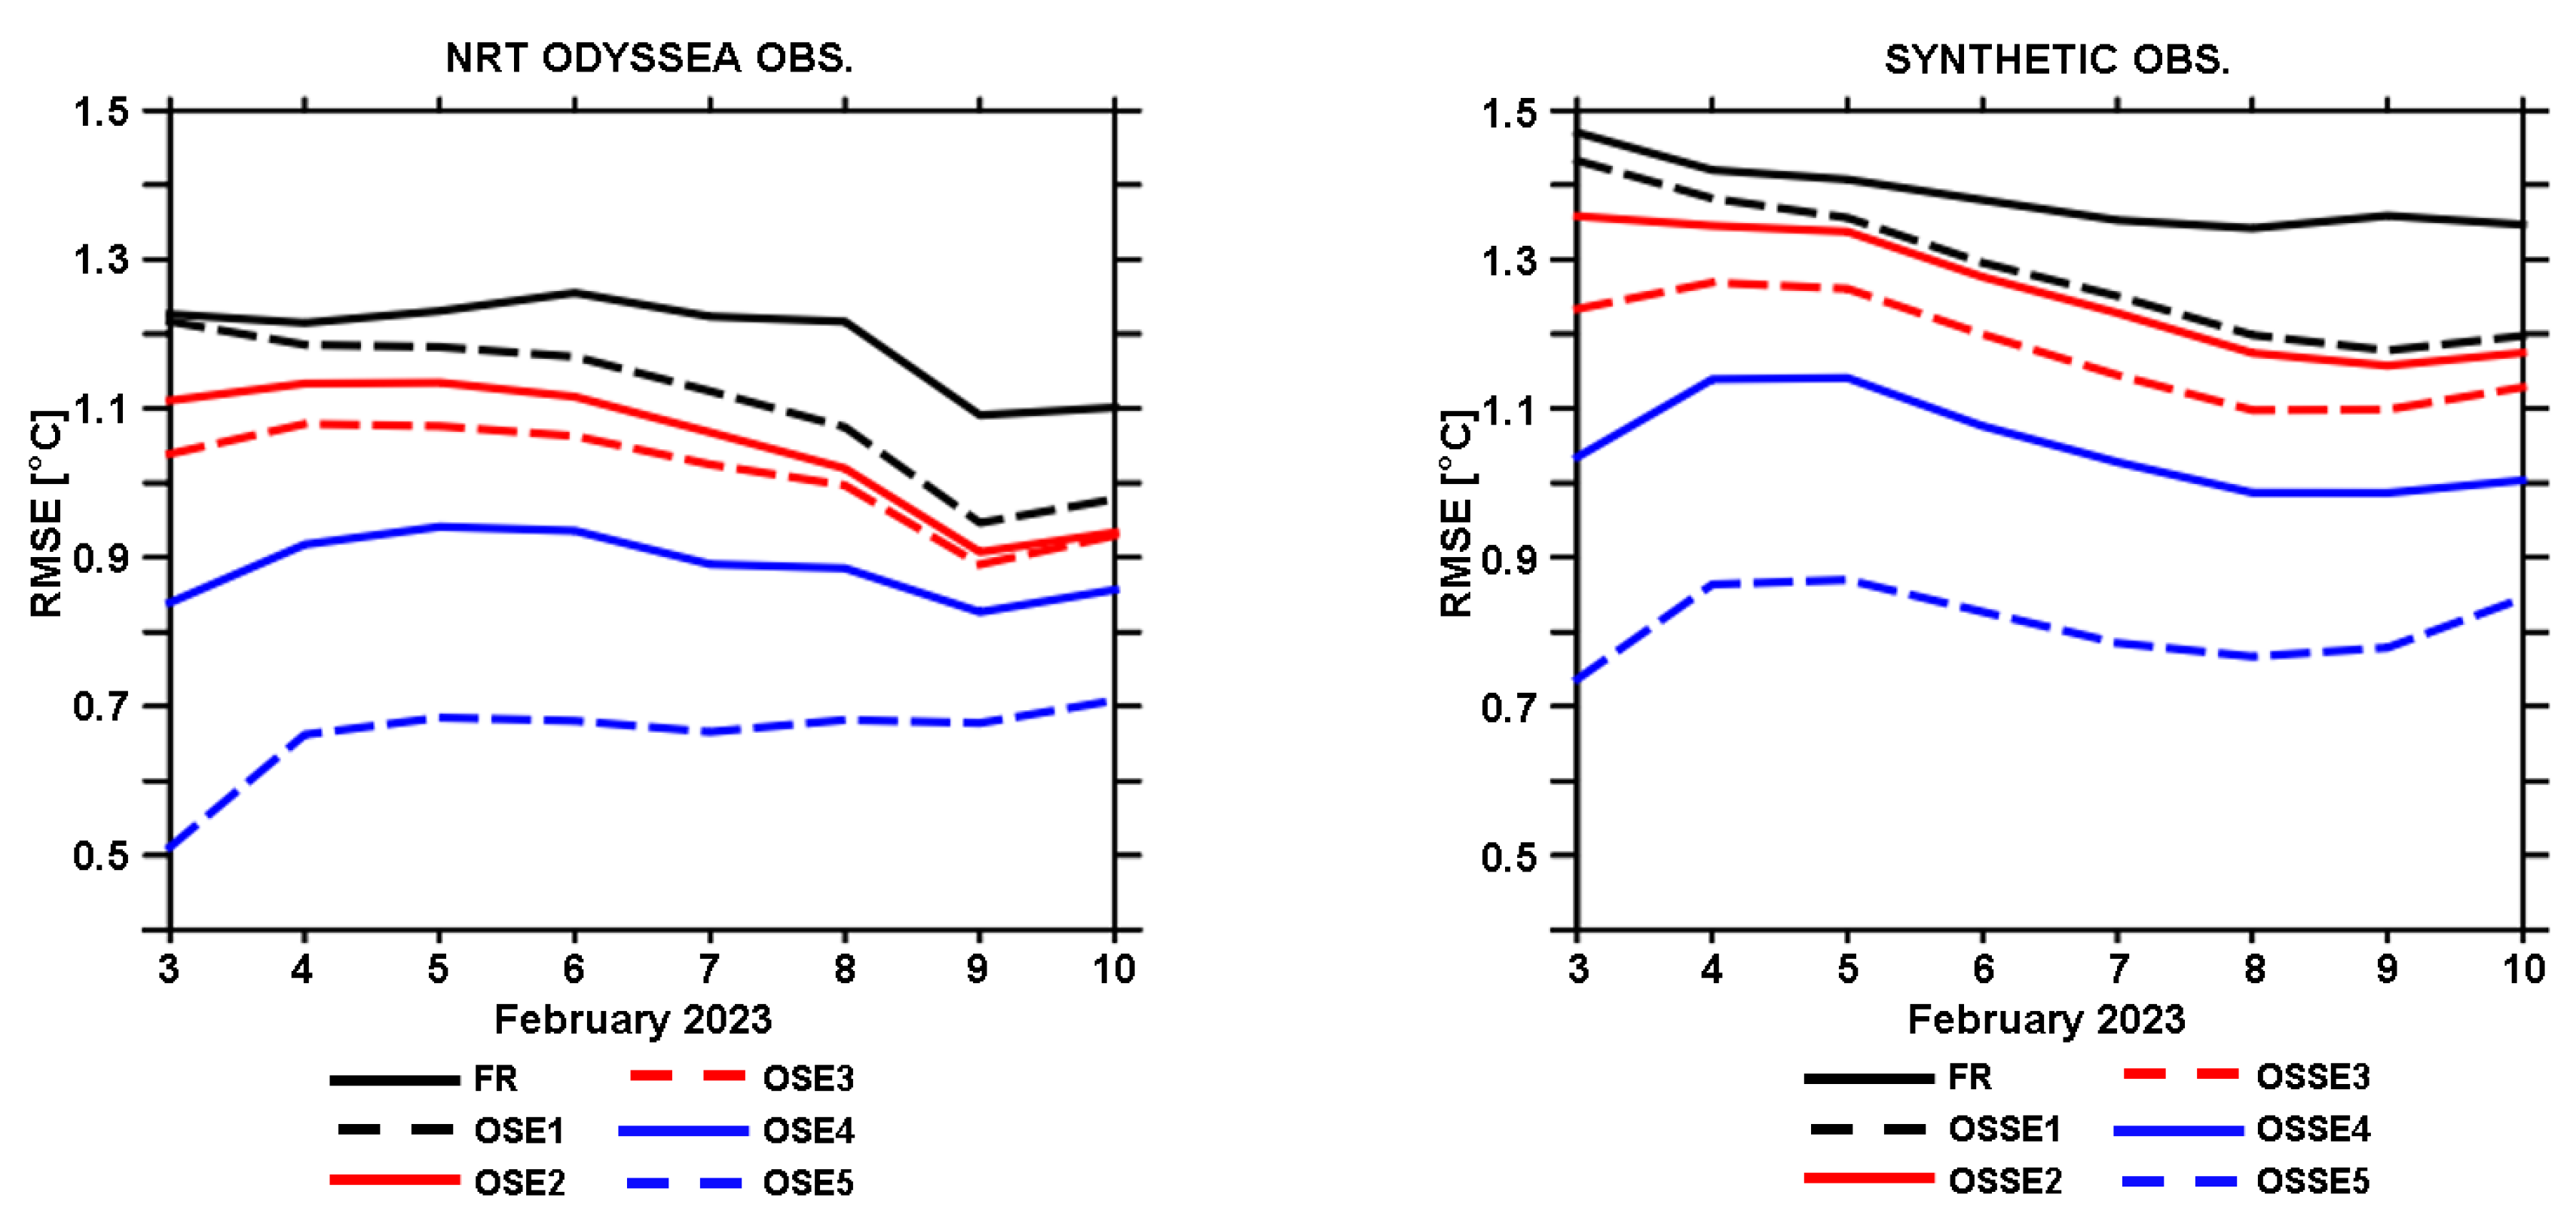
\includegraphics[width=15.0cm]{figures/fig2.6.png}
    \caption{On the left, the SST error over time of the FR and experiments OSE1 to OSE5, referenced in \bCref{tab:exps_2.1}, with respect to the NRT ODYSSEA satellite product. On the right, the SST error of the FR and experiments OSSE1 to OSSE5 with respect to the NR. The experiments were integrated for an additional seven days following the update on 3 February.}
    \label{fig:rmsenrt_2.6}
\end{figure}

A detailed analysis of \bCref{fig:rmsenrt_2.6} provides important insights into the OSSE system's behaviour following the updates. Most likely due to the random multiplicative factor that increases the observation errors, the RMSE of the FR with respect to the NR is consistently higher than the RMSE relative to the satellite observations. However, the emphasis here is not on this absolute difference, but on the relative consistency across experiments. Both OSE and OSSE configurations exhibit a clear, monotonic reduction in RMSE as the number of assimilated observations increases. The temporal evolution also shows that, as expected, assimilating a large number of observations produces a gradual increase in RMSE in the days following the update, whereas assimilating only a few points tends to increase the RMSE at analysis time, with the resulting dynamical inconsistencies causing more harm than benefit.

Notably, the OSSE experiments closely mirror the behaviours of their corresponding OSE counterparts over time, despite relying solely on synthetic data. For each observation count, the RMSE curves of the OSSEs follow trends that are closely aligned with those of the OSEs, indicating that the synthetic updates generate corrections in the model state that are dynamically comparable to those achieved through the assimilation of real satellite observations. This agreement is particularly clear when comparing experiments configured with the same number of assimilated observations (e.g., OSE3 versus OSSE3). Comparable consistency was also found when repeating the experiments with the Reprocessed satellite product, reinforcing that the OSSE system responds similarly when assimilating equivalent datasets. Had the results from the Reprocessed product diverged substantially from those using the NRT ODYSSEA data, it could have indicated shortcomings in the system's design and the need for further refinement.

In addition to the temporal RMSE analysis, Taylor diagrams were used to evaluate the similarity between the forecast fields and the reference data. These were generated for two instants: the day of the EnOI update step (3 February) and seven days afterward (10 February). \bCref{fig:taylornrt_2.7} presents the results for the experiments based on the NRT ODYSSEA satellite product. In line with previous RMSE-based assessment, the overall patterns in the diagrams are consistent. The most relevant aspect lies not in the precise values, but in the comparative behaviour of OSSEs relative to OSEs. The satellite data (SAT\_NRT in the figure) and the NR serve as reference anchors, with SAT\_NRT exhibiting a higher standard deviation, reflecting its origin as a gridded observational product. As observations are progressively assimilated into the FR, the forecast state converges toward the reference: the OSE experiments (red markers) move closer to SAT\_NRT, while the OSSE experiments (yellow markers) approach the NR. Although the OSSEs show slightly higher root mean square differences (RMSD) than the OSEs, consistent with the RMSE trends, both follow remarkably similar trajectories in terms of correlation and RMSD reduction. This convergence was also evident in the experiments using the Reprocessed satellite product.

\begin{figure}[H]
    \centering
    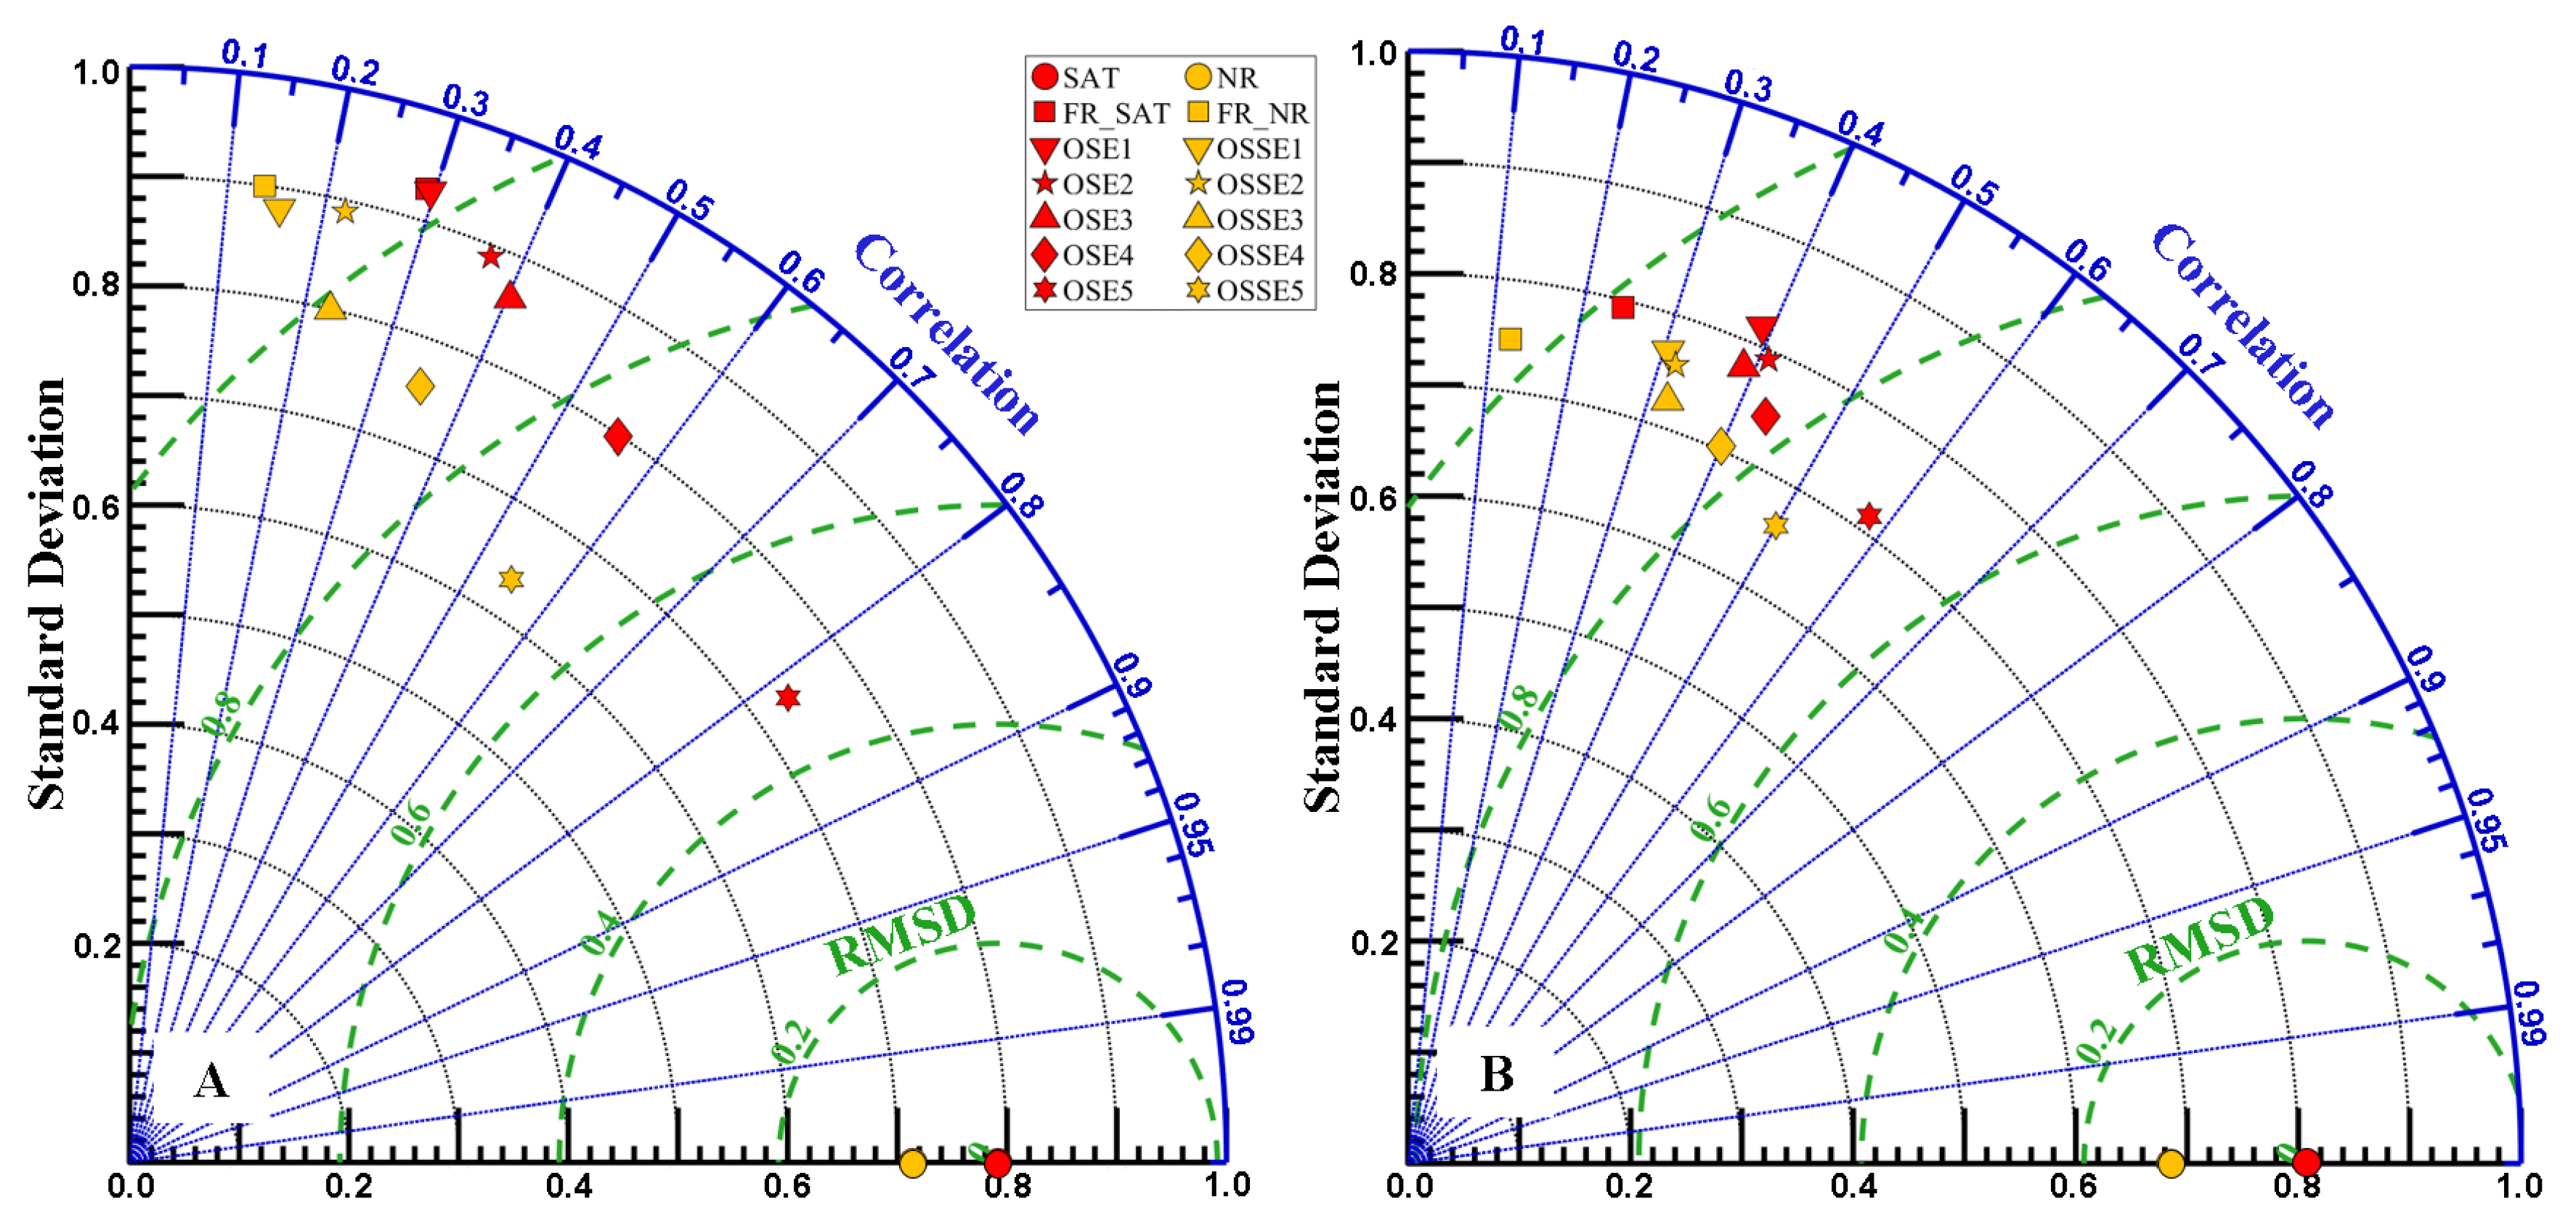
\includegraphics[width=16.0cm]{figures/fig2.7.png}
    \caption{The Taylor diagrams present the statistical properties (standard deviation, correlation, and root mean square difference, RMSD) for OSE1-OSE5 and OSSE1-OSSE5, as well as the Free Run (FR\_SAT) relative to the NRT ODYSSEA satellite data (SAT) and the Free Run (FR\_NR) relative to the Nature Run (NR). Panel~(\textbf{A}) shows the results immediately after the EnOI update, and Panel~(\textbf{B}) shows the results seven days later.}
    \label{fig:taylornrt_2.7}
\end{figure}

Finally, an additional metric was used to further assess the system's behaviour: the Murphy Skill Score (MSS), as defined in \bCref{eq:cp2_murphyss}. For the OSE experiments, the NR values in the equation were replaced by the corresponding satellite product, which served as the observational reference. In the OSSE experiments, the NR values remained the reference dataset, reflecting the synthetic nature of these experiments. The results for the experiments based on the NRT ODYSSEA satellite product are shown in \bCref{fig:murphy_2.8}. Each panel illustrates how the MSS varies with the number of assimilated observation points, with the left panel representing the moment immediately after the EnOI update (3 February) and the right panel representing the results from the sampling seven days later (10 February).

As expected, the skill score generally increases as more observations are assimilated, indicating enhanced forecast accuracy. More importantly, the OSSE curves follow the same upward trend as their OSE counterparts, reaffirming the system's consistency. The analysis MSS increases even when a large number of data points is assimilated, whereas the forecast MSS is less sensitive to the number of observations, possibly being hampered by the quality of other inputs, such as lateral and surface boundary conditions. No specific benchmark value for the MSS was sought; rather, the objective was to confirm that OSSE experiments respond similarly to OSEs in terms of performance improvement. Overall, the results demonstrate that the OSSE system developed in this study is internally consistent, sensitive to observation density, and capable of realistically reproducing the correction patterns expected from real-world assimilation. This provides strong evidence of its suitability for assessing the potential impact of future observational strategies, such as those envisioned under the NAUTILOS initiative.

\begin{figure}[H]
    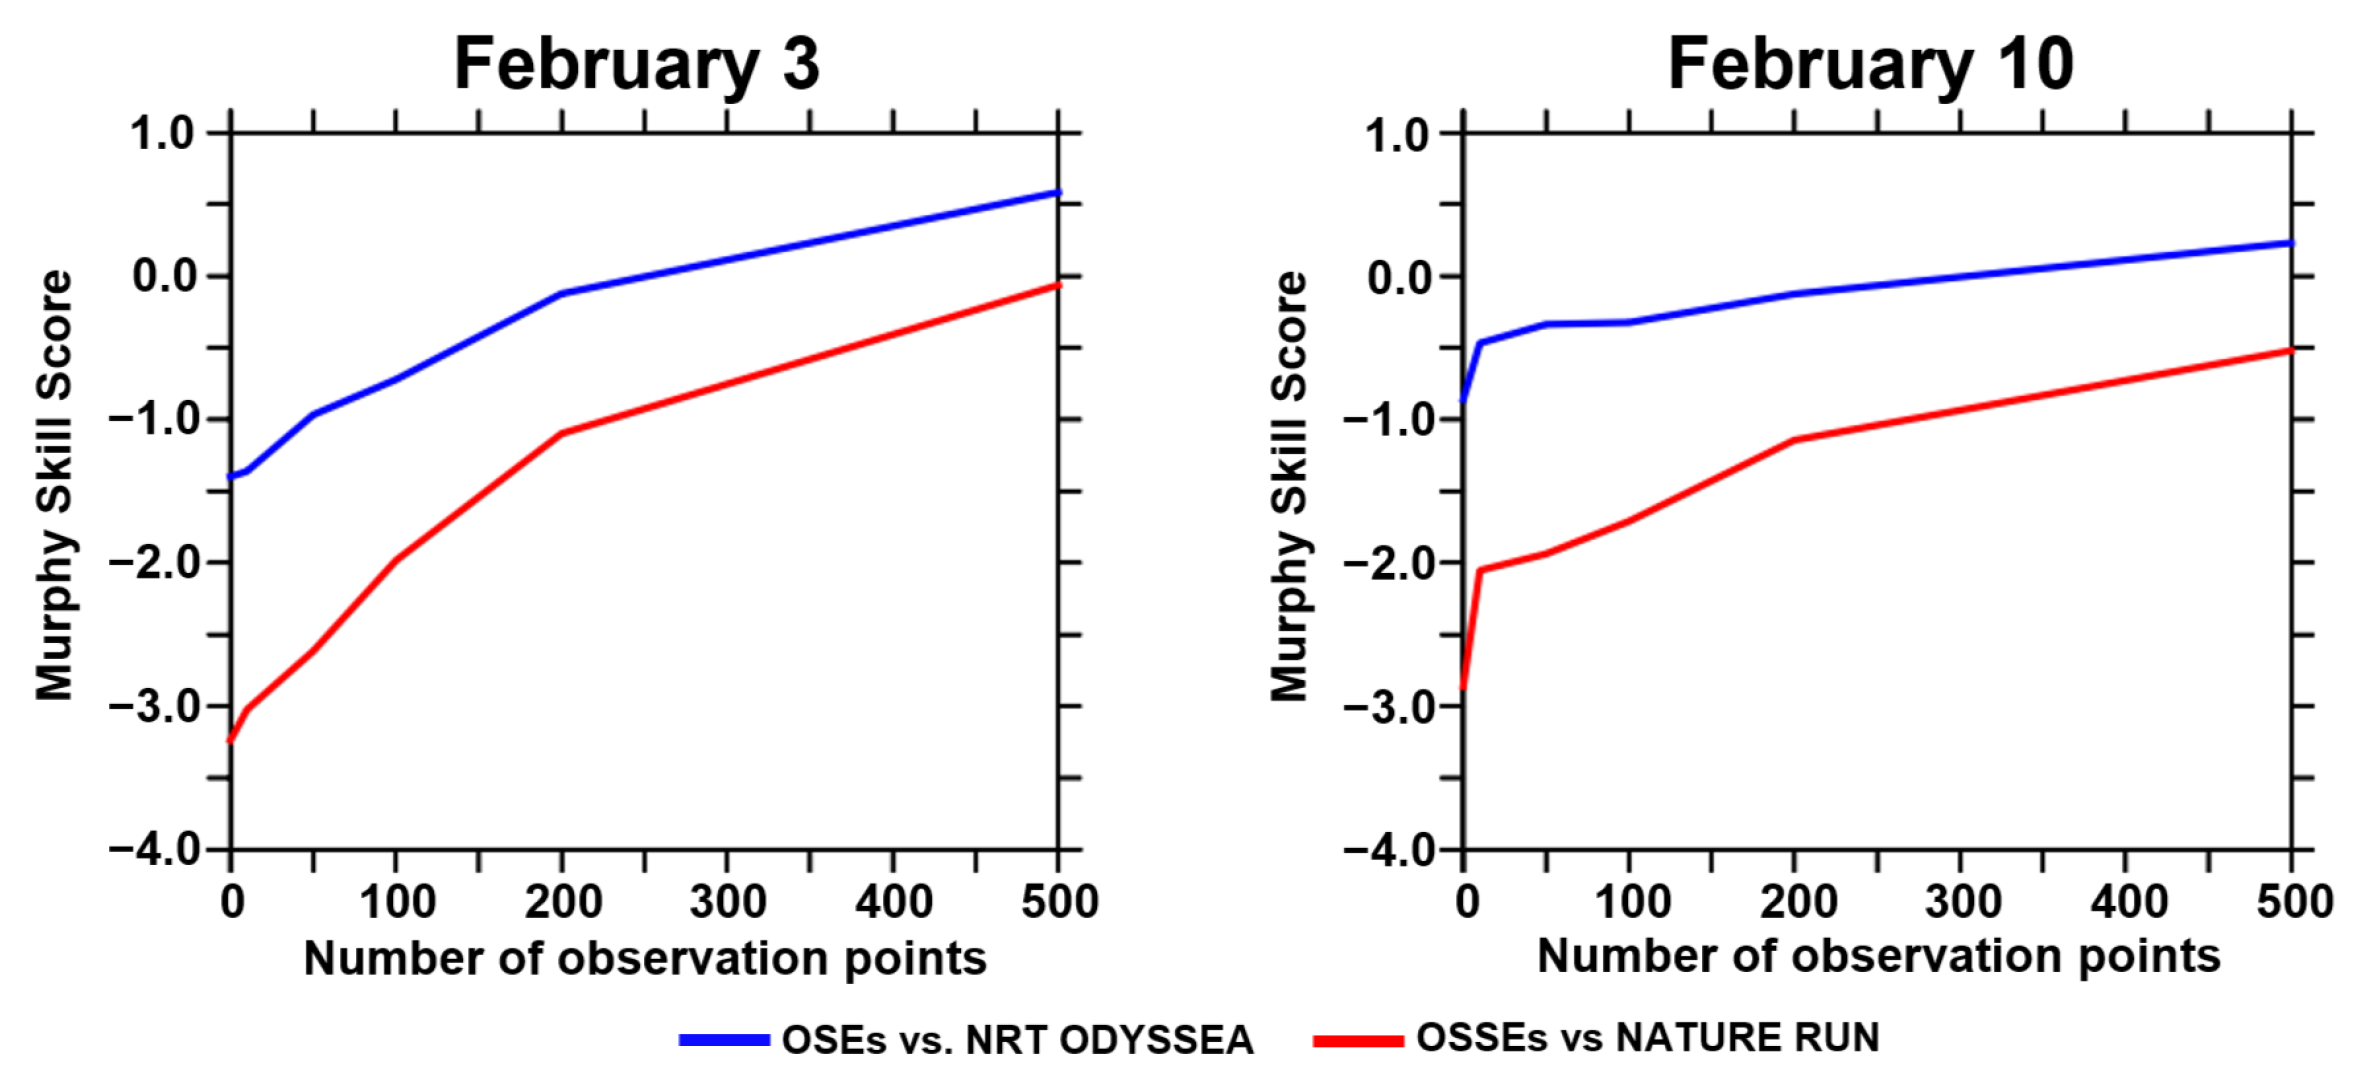
\includegraphics[width=15.0cm]{figures/fig2.8.png}
    \caption{Murphy Skill Score (MSS) for experiments based on the NRT ODYSSEA satellite product. Blue lines indicate OSE experiments, with skill scores computed relative to their satellite-based reference data; red lines indicate OSSE experiments, computed relative to the NR. The left panel shows MSS immediately after the EnOI update (3 February), and the right panel shows MSS seven days later (10 February).}
    \label{fig:murphy_2.8}
\end{figure}

\section{Conclusions} \label{sec:ossedesign_conclude}
A practical framework for assessing the possible influence of new observation systems on model forecasts before their actual deployment is provided by Observation System Simulation Experiments (OSSEs). Within this context, the main objective of this study was to design and validate an OSSE system tailored to the operational model of the Algarve coast, SOMA. The system was developed using the fraternal twins approach, in which two configurations of the same model, MOHID, were used to simulate the Nature Run (NR) and the Forecast Model (FM).

In the NR, SOMA's original operational configuration was used. In contrast, the FM was modified to a lower-resolution grid and did not include weekly adjustments from outer conditions. For this reason, the FM was also referred to as the Free Run (FR) in the proposed OSSE system. Data assimilation was carried out using the EnOI scheme, which was chosen for its balance between computational efficiency and representativeness of ensemble-based statistics. At this stage, assimilation was limited to surface observations, both due to the current configuration of the DA system, which still requires further adaptation to support 3D assimilation with SOMA, and to ensure consistency with the operational satellite-based products used in the Observing System Experiments (OSEs).

As recommended in the literature, an OSSE system should be evaluated against a comparable OSE system in order to ensure that the former does not produce unrealistic results when assessing new observations. In this study, such a comparison was made using two distinct L4 satellite products for SST from CMEMS: the NRT ODYSSEA product and the Reprocessed dataset. These products served as references for the OSE experiments, while the corresponding OSSEs assimilated synthetic SST observations derived from the NR. The results confirmed that the OSSE system responded consistently across both satellite references, as demonstrated by the RMSE evolution over time, Taylor diagrams, and Murphy Skill Score; these results support its robustness and reliability for future impact assessments.

A key aspect of the methodology is the emulation of realistic observational errors in the synthetic data, which ensures that the assessment of new data streams reflects the uncertainties of real-world applications. This was achieved by generating pseudo-random fields, using a spatial correlation factor across the NR grid, and scaling by satellite-derived error data. The result is a flexible framework that preserves the statistical structure of real observation errors and can be used to test different error magnitudes in the future. Although the experiments presented were tailored to SOMA and the Algarve region, the methodological framework is not tied to SOMA specifically. The generation of synthetic observations and their associated error fields allows for straightforward transfer to other coastal models and regional contexts, broadening the model's applicability and making it useful as a base model for evaluating emerging observing systems beyond that presented in the present case study. 

The results presented here indicate that the SOMA OSSE system is consistent, sensitive to the number of observations used in the update step, and capable of realistically emulating synthetic observation errors. As such, it provides a solid foundation for future studies aimed at assessing the impact of emerging observation strategies in the Algarve region, including those being developed under the NAUTILOS project. Beyond its immediate application, the system also paves the way to broader developments, such as more in-depth research into the correlation between the SST and salinity state variables of the model, which could enhance the system's robustness by enabling more advanced multivariate assimilation strategies.

This work also constitutes a very significant milestone in SOMA's operational forecasts: the adaptation and integration of a DA system to improve the model state variables, including real satellite observations. However, the restriction to surface-only assimilation remains a critical limitation of the current system. Future developments should prioritize the integration of the EnOI scheme with real-time forecasts and the expansion of its scope to encompass additional observation types, such as satellite altimetry and 3D in situ fields like those obtained by autonomous platforms, including the AUV missions already operational in the region \parencite{cima2024soma}. In addition, a systematic sensitivity analysis of the weighting coefficient $\alpha$ will be an essential step in optimizing the balance between background error structures and observational impact, ensuring a more robust assimilation framework. In this sense, the present study should be seen as a first step in the development of a more comprehensive DA framework that will culminate in a significant enhancement of the operational monitoring capacity along the Algarve coast.

\section{Supplementary Materials} \label{sec:cp2_supp}
\begin{figure}[H]
   \centering
   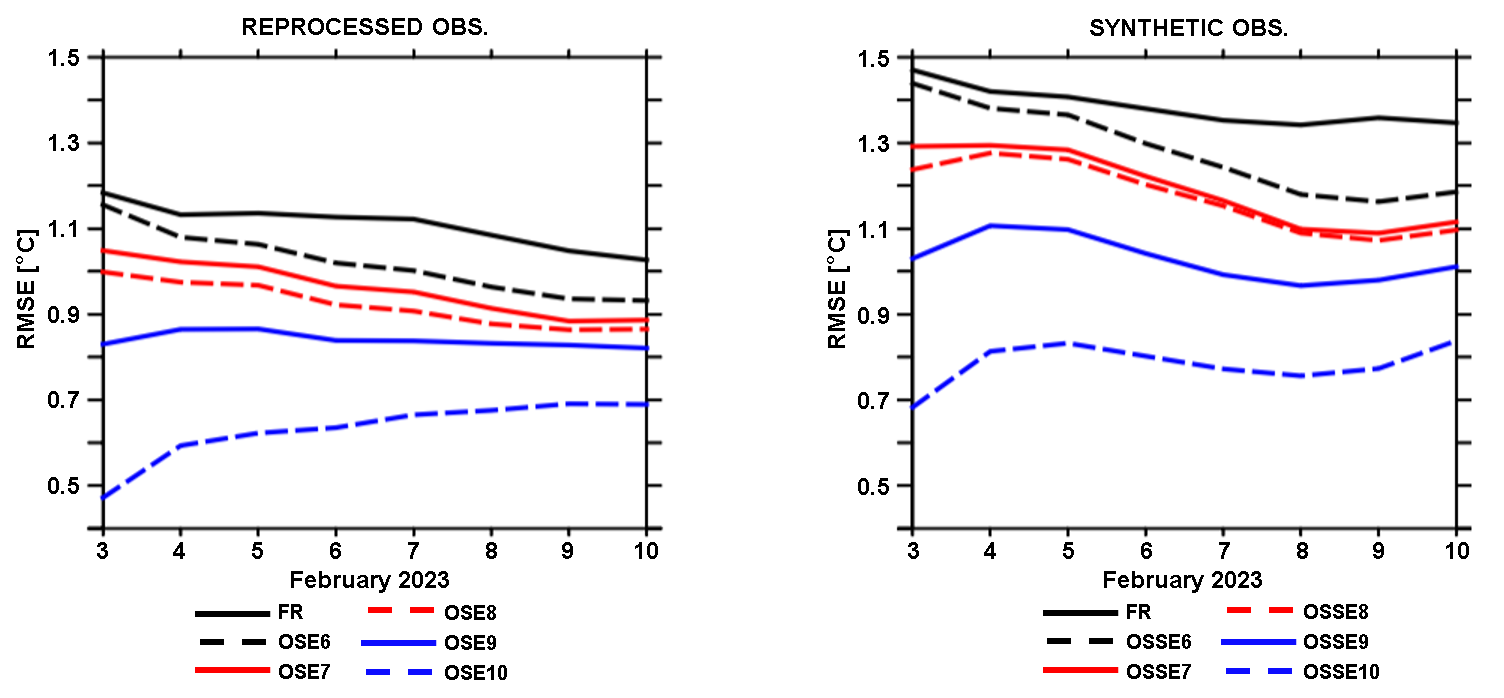
\includegraphics[width=15.0cm]{figures/fig2.9.png}
   \caption{On the left, the SST error over time of the FR and experiments OSE6 to OSE10, referenced in \bCref{tab:exps_2.1}, with respect to the Reprocessed satellite product. On the right, the SST error of the FR and experiments OSSE6 to OSSE10 with respect to the NR. The experiments were integrated for an additional seven days following the update on 3 February.}
   \label{fig:rmserep_2.9}
\end{figure}


\section{Data Availability Statement}
The operational data from the Algarve modelling system (SOMA) are openly available at \href{https://doi.org/10.34623/tx0z-bb23}{https://doi.org/10.34623/tx0z-bb23}.

\section{Appendix A} \label{sec:ossedesign_appxA}
This appendix details the core metrics used to evaluate the Forecast Model (FM) against the Nature Run (NR). The same equations are applied to assess (1) the FM against actual observation data, (2) OSSE experiments against the NR, and (3) OSE experiments against observational data.

\subsection{Spatially Integrated Averages and Standard Deviations}
A straightforward comparison between the models can be accomplished by calculating the instantaneous spatial averages (\textit{AVG}) and standard deviations (\textit{STD}) of the NR and FM. The resulting data can then be utilized to construct a time series of model evolution. The parameters are defined as follows:

\begin{equation}\label{eq:cp2_avg}
	AVG(t_{i}) = \frac{\Sigma_{\text{domain}}\theta(t_{i})}{N},
\end{equation}
\begin{equation}\label{eq:cp2_std}
	STD(t_{i}) = \sqrt{\frac{\Sigma_{\text{domain}} \Bigl( \theta(t_{i})-AVG(t_{i}) \Bigr)^2}{N}}.
\end{equation}

In the previous equations, $\theta$ is the analyzed variable at time $t_i$, and $N$ the number of grid cells. Values can represent instantaneous outputs or averages within a time window centered on $t_i$, with both the window length and sampling frequency (e.g., daily or weekly) depending on the process and region. Spatial sums may cover the full 3D field or a chosen 2D layer, such as the surface. The time series obtained from \textit{AVG} (\bCref{eq:cp2_avg}) and \textit{STD} (\bref{eq:cp2_std}) offer a straightforward means of comparing the FM against the NR through time. The same diagnostics can be extended to observational datasets (e.g., L4 SST or SSH data products), ensuring that the model's statistical behaviour is consistent with real-world conditions.

\subsection{Spatially Integrated RMSE}
The time series of the instantaneous spatially integrated root mean square error (\textit{RMSE}) is an effective preliminary indicator of the forecast evolution in relation to the NR and observations. This parameter is defined by the following equation:

\begin{equation}\label{eq:cp2_rmse}
	RMSE(t_i) = \sqrt{\frac{\Sigma_\text{domain} \Bigl( \theta_{FM}(t_i) - \theta_{NR}(t_i) \Bigr)^2}{N}}.
\end{equation}

In the last equation, $\theta_{NR}$ and $\theta_{FM}$ represent the variables from the Nature Run and the Forecast Model, respectively, at time $t_i$, while $N$ is the number of grid cells considered. As with \textbf{Equations}~\bref{eq:cp2_avg} and~\bref{eq:cp2_std}, $\theta$ may correspond either to instantaneous outputs or to averages within a time interval centred on $t_i$, with the choice of interval and sampling frequency (e.g., daily or weekly) depending on the process and region under study. The spatial integration can also be carried out over the full 3D domain or restricted to a 2D layer. Since the NR often employs a finer spatial resolution than the FM does to reduce the risk of the \textit{identical twins} problem, it is standard practice to average the NR fields onto the FM grid prior to computing \textit{RMSE}.

\subsection{Temporally Integrated Averages and Standard deviations}
The previous indicators provide a global overview of the temporal evolution of the solutions, yet they do not allow a spatial evaluation. To address this limitation, temporally integrated indicators for each grid point can be employed. The temporally integrated average is computed as follows:

\begin{equation}\label{eq:cp2_avgt}
    AVG(i,j,k) = \frac{\sum_{t_i=0}^{T}\theta(i,j,k)}{N},
\end{equation}

\noindent where $\theta$ denotes the analysed variable, either from the Forecast Model or the NR, evaluated at grid point $(i,j,k)$, while $T$ is the number of time steps included. The values of $\theta$ may correspond to instantaneous outputs or to averages over a time interval centred on $t_i$. Using the same approach, the standard deviation can be derived according to \bCref{eq:cp2_stdt}:

\begin{equation}\label{eq:cp2_stdt}
    STD(i,j,k) = \sqrt{\frac{\sum_{t_i=0}^{T} \Bigl( \theta(i,j,k) - AVG(i,j,k) \Bigr)^2}{N}}.
\end{equation}

Horizontal and vertical maps can be plotted from the indicators in \textbf{Equations}~\bref{eq:cp2_avgt} and~\bref{eq:cp2_stdt}, which provide a general idea of the spatial behaviour of the model statistics.

\subsection{Temporally Integrated RMSE}
The temporally integrated \textit{RMSE} between the forecast and the reference NR can be calculated using the same logic employed for the previous indicators. This allows the plotting of horizontal maps of each layer or vertical cuts, which provide a general overview of the spatial distribution of forecast deviations relative to the NR. It is computed by the following:

\begin{equation}\label{eq:cp2_rmset}
    RMSE(t_i) = \sqrt{\frac{\sum_{t_i=0}^{T} \Bigl( \theta_{FM}(i,j,k) - \theta_{NR}(i,j,k) \Bigr)^2}{N}}.
\end{equation}

\subsection{Murphy Skill Score}
The metrics described in \Cref{sec:ossedesign_appxA} provide a general characterization of the NR and FM and a simple way to compare them. However, the literature also recommends the use of more sophisticated statistical metrics, such is the Murphy Skill Score (\textit{MSS}):

\begin{equation}\label{eq:cp2_murphyss}
    MSS = \rho^2 - \left[ \rho - \frac{\sigma_{FM}}{\sigma_{NR}} \right]^2 - \left[ \frac{\overline \theta_{FM}-\overline \theta_{NR}}{\sigma_{NR}} \right]^2.
\end{equation}

The \textit{MSS} can be evaluated either over the full grid or individually at each grid cell for a selected time period, thereby yielding a spatial distribution of predictive performance. In \bCref{eq:cp2_murphyss}, $\rho$ is the correlation between the NR and FM, $\sigma$ is the standard deviation, and $\overline{\theta}$ represents the average of the variable analysed. Following \textcite{murphy1988skill}, \textit{MSS} values vary between $-\infty$ and 1: a score of 1 corresponds to a perfect forecast, 0 indicates no improvement relative to the reference, and negative values denote performance worse than that of the reference. Intermediate values $(0 < MSS < 1)$ indicate increasing levels of forecast improvement.

\subsection{Taylor Diagrams} \label{subsec:cp2_taylor}
The Taylor Diagram \parencite{taylor2001summarizing} is a graphical tool developed to summarize the performance of models by combining three statistical metrics---correlation, root mean square difference (\textit{RMSD}), and standard deviation---into a single and interpretable plot. It provides a compact way to visualize and compare the agreement between the forecast output and the reference NR, where each comparison (or each OSSE) is represented as a point on a polar coordinate system. The azimuthal position of each point reflects the correlation between FM and NR, while the radial distance from the origin represents the pattern's standard deviation, and the distance from the reference point shows the RMSD. Thus, the diagram offers a rapid method of evaluating the accuracy of the forecast model.

The distinction between \textit{RMSE} and \textit{RMSD} lies in their respective focuses. \textit{RMSE} is a broader measure of overall accuracy, capturing both the mean difference (bias) and variability between the forecast and NR. In contrast, \textit{RMSD} removes the bias first, allowing it to emphasize discrepancies in the shape and phase of the spatial or temporal structure and variability of the dataset. Thus, it is defined by the following equation:

\begin{equation}\label{eq:cp2_rmsd}
    RMSD = \sqrt{\frac{\sum_{i=1}^N \Bigl( (\theta_{FM_i} - \overline\theta_{FM}) - (\theta_{NR_i} - \overline\theta_{NR}) \Bigr)^2}{N}},
\end{equation}

\noindent where $\theta$ is the analysed variable in FM and NR; $\overline\theta$ is the average of that variable; and $N$ is the number of grid cells used. In general, the closer the forecast result is to the NR, the better the model performance.
 
\section{Appendix B} \label{sec:ossedesign_appxB}
The general formulation of the Ensemble Optimal Interpolation (EnOI) can be introduced through the standard analysis equation of a Data Assimilation (DA) problem, expressed in \textbf{Equations}~(\bref{eq:cp2_daprob}) and~(\bref{eq:cp2_daK}), where the time index is omitted for clarity:

\begin{equation}\label{eq:cp2_daprob}
	\mathbf{x}^a=\mathbf{x}^b+\mathbf{K} \left( \mathbf{y}-\mathbf{Hx}^b \right),
\end{equation}

\begin{equation}\label{eq:cp2_daK}
	\mathbf{K}=\mathbf{PH}^T \left[ \mathbf{HPH}^T+\mathbf{R} \right]^{-1}.
\end{equation}

\bCref{eq:cp2_daprob} provides the model state update in $\mathbf{x}^a$. The current state of the model, or the background, is denoted by $\mathbf{x}^b$ and, together with the analysis, they are m-dimensional vectors of real numbers, i.e., $\left( \mathbf{x}^a,\mathbf{x}^b \right) \in \mathbb{R}^m$. The state vectors typically contain the values at all grid cells of all variables being updated in the assimilation process, such as velocity components, temperature, salinity, or SSH, although the specific variables included depend on the configuration and objectives of the system. The observation vector is given by $\mathbf{y} \in \mathbb{R}^d$ and $\mathbf{H} \in \mathbb{R}^{d \times m}$ is a matrix which serves as an operator to map the background vector to the observations' space.

In \bCref{eq:cp2_daK} the superscripts $^T$ indicate a transposed matrix, $\mathbf{K} \in \mathbb{R}^{m \times d}$ is the matrix of weights, akin to the Kalman gain in the Ensemble Kalman Filter (EnKF), $\mathbf{P} \in \mathbb{R}^{m \times m}$ is the background error covariance matrix, and $\mathbf{R} \in \mathbb{R}^{d \times d}$ is the observation error covariance matrix. From the two equations and in the event that the uncertainty associated with the model is significantly smaller than that associated with the observations (i.e., $\mathbf{P}<<\mathbf{R}$), the weights approach zero. Consequently, the analysis in \bCref{eq:cp2_daprob} practically becomes the value of the background. Conversely, if the observations are more reliable than the model (i.e., $\mathbf{R}<<\mathbf{P}$), then more weight is given to the observations.

If the analysis equation is to be solved, some definitions must be given. Firstly, the matrix holding the static ensemble members of the background is given by $\mathbf{E}$ in \bCref{eq:cp2_ensemble}:

\begin{equation}\label{eq:cp2_ensemble}
	\mathbf{E}=\left( \mathbf{x_1},\mathbf{x_2},\cdots,\mathbf{x_N} \right)\in\mathbb{R}^{m\times N},
\end{equation}

\noindent where $N$ is the number of ensemble members, each one an m-dimensional state vector. With that, the ensemble anomaly ($\mathbf{X'}$) is defined as the following:

\begin{equation}\label{eq:cp2_anomaly}
	\mathbf{X'}=\mathbf{E}-\overline{\mathbf{E}},
\end{equation}

\noindent where $\overline{\mathbf{E}}$ is the ensemble mean. Then, the ensemble covariance matrix $\mathbf{P}$ can be defined as

\begin{equation}\label{eq:cp2_encov}
	\mathbf{P}=\frac{\mathbf{X'X'}^{T}}{N-1}.
\end{equation}

Moving to the measurements vector $\mathbf{y}$ in \bCref{eq:cp2_daprob}, an ensemble of perturbed observations must be introduced into the system to ensure that the ensemble analysis properly accounts for the measurement uncertainty and maintains consistency with the computation of the Kalman gain. The perturbation is defined by \bCref{eq:cp2_enobs}:

\begin{equation}\label{eq:cp2_enobs}
	\mathbf{y_i}=\mathbf{y}+\epsilon_i, \quad 1\leq i\leq N,
\end{equation}

\noindent where $\epsilon_i$ is the simulated random measurement error, drawn from a distribution with zero mean and a covariance that matches the observation error covariance matrix $\mathbf{R}$ in \bCref{eq:cp2_daK}. In this way, the perturbed observations can be stored in the following observation matrix:

\begin{equation}\label{eq:cp2_obspertub}
    \mathbf{Y}=\left( \mathbf{y_1},\mathbf{y_2},\cdots,\mathbf{y_N} \right)\in\mathbb{R}^{d\times N}.
\end{equation}

With the previous statements, it is possible to replace the error covariance matrices in the analysis $\mathbf{x}^a$ and in $\mathbf{K}$ by their ensemble representation to obtain the ensemble of updated states ($\mathbf{E}^a$):

\begin{equation}\label{eq:cp2_enkf}
    \mathbf{E}^a=\mathbf{E} + \mathbf{X'X'}^T \mathbf{H}^T \left[ \mathbf{HX'X'}^T \mathbf{H}^T +(N-1) \mathbf{R}\right]^{-1} \left( \mathbf{Y}-\mathbf{HE} \right).
\end{equation}

\bCref{eq:cp2_enkf} shows the general formulation of the EnKF analysis scheme, which includes updating each member of the ensemble and integrating the model $N$ times to calculate the error covariance matrix $\mathbf{P}$. However, in the EnOI, the analysis is computed only for one single model state, so the last equation can be rewritten as follows:

\begin{equation}\label{eq:cp2_enoi}
    \mathbf{x}^a=\mathbf{x}^b + \alpha\mathbf{X'X'}^T \mathbf{H}^T \left[ \alpha\mathbf{HX'X'}^T \mathbf{H}^T +(N-1) \mathbf{R}\right]^{-1} \left( \mathbf{y}-\mathbf{Hx}^b \right).
\end{equation}

In \bCref{eq:cp2_enoi}, the parameter $\alpha\in(0,1]$ is introduced to tune the weight given to the ensemble background error covariance relative to the observation error covariance \parencite{evensen2003ensemble}. Since EnOI employs a stationary ensemble to approximate background error statistics, the background variance can sometimes be overestimated due to the long-term sampling of model states. The scaling factor $\alpha$ mitigates this issue by reducing the ensemble-based covariance contribution to a level that better represents the actual forecast uncertainty at the time of assimilation. When $\alpha$ approaches zero, the effective observation error variance is inflated, leading the analysis to converge toward the background state ($\mathbf{x}^a \approx \mathbf{x}^b$). Conversely, as it approaches one, the ensemble covariance is fully retained, allowing the observations to exert a stronger influence on the analysis update.
